% !TEX program = xelatex
% ============================================================================
%  Bachelor Thesis - Royal University of Phnom Penh
%  "Explainable AI for Automated Grading of Khmer Language Short-Answer
%   Questions in Education"
%
%  COMPILE WITH XeLaTeX (required for Khmer script).
%  Sequence:  xelatex -> bibtex -> xelatex -> xelatex
%  On Overleaf: Menu -> Compiler -> XeLaTeX. See README.md.
% ============================================================================
\documentclass[12pt,a4paper,oneside]{report}

% ---- Page geometry (RUPP-style binding margin) ----
\usepackage[a4paper,left=3.5cm,right=2.5cm,top=2.5cm,bottom=2.5cm]{geometry}

% ---- Fonts & languages (XeLaTeX) ----
\usepackage{fontspec}
\usepackage{polyglossia}
\setdefaultlanguage{english}
\setotherlanguage{khmer}
% Latin body font (Times-like; bundled on Overleaf/TeX Live):
\setmainfont{TeX Gyre Termes}
% Khmer font - upload "Noto Sans Khmer" to the Overleaf project if not present.
\newfontfamily\khmerfont[Script=Khmer]{Noto Sans Khmer}

% ---- Core packages ----
\usepackage{amsmath,amssymb}
\usepackage{graphicx}
\usepackage{booktabs}
\usepackage{array}
\usepackage{multirow}
\usepackage{longtable}
\usepackage{setspace}
\usepackage[font=small,labelfont=bf]{caption}
\usepackage{enumitem}
\usepackage{xcolor}
\usepackage{tikz}
\usetikzlibrary{arrows.meta,positioning}
\usepackage{fancyhdr}
\usepackage[round,authoryear]{natbib}
\usepackage[hidelinks]{hyperref}

% ---- Citation style (author-year, RUPP/APA-like) ----
\bibliographystyle{apalike}

% ---- Layout niceties ----
\onehalfspacing
\setlength{\parskip}{4pt}
\graphicspath{{figures/}}
\renewcommand{\arraystretch}{1.15}

% Running header
\setlength{\headheight}{14.5pt}
\pagestyle{fancy}
\fancyhf{}
\fancyhead[L]{\small\leftmark}
\fancyhead[R]{\small\thepage}
\renewcommand{\headrulewidth}{0.4pt}

% Convenience macro for inline Khmer
\newcommand{\km}[1]{\textkhmer{#1}}

\begin{document}

% ============================ FRONT MATTER ============================
\pagenumbering{roman}
% ---- Title page (RUPP format). Replace every [bracketed] placeholder. ----
\begin{titlepage}
\centering
\thispagestyle{empty}

{\large \km{សាកលវិទ្យាល័យភូមិន្ទភ្នំពេញ}\par}
{\large ROYAL UNIVERSITY OF PHNOM PENH\par}
\vspace{0.4cm}
{\normalsize Faculty of Engineering \,/\, [Department of Data Science and Engineering]\par}

\vfill

{\large \km{ប្រធានបទនិក្ខេបបទ}\par}
\vspace{0.3cm}
{\Large\bfseries Explainable AI for Automated Grading of\\[2pt]
Khmer Language Short-Answer Questions in Education\par}

\vspace{1.0cm}
{\normalsize A Thesis\\
In Partial Fulfilment of the Requirements for the Degree of\\
\textbf{Bachelor of [Data Science and Engineering]}\par}

\vfill

{\large Phork Norak\par}
\vspace{0.2cm}
{\normalsize Supervisor: Dr. Khim Chamroeun\par}

\vspace{0.8cm}
{\normalsize [Month] 2026\par}

\end{titlepage}
\clearpage

% ---- Examination committee page (replace placeholder names) ----
\thispagestyle{empty}
\begin{center}
{\large \km{សាកលវិទ្យាល័យភូមិន្ទភ្នំពេញ}\par}
{\large ROYAL UNIVERSITY OF PHNOM PENH\par}
\vspace{0.3cm}
{\Large\bfseries Explainable AI for Automated Grading of\\[2pt]
Khmer Language Short-Answer Questions in Education\par}
\vspace{0.6cm}
{\normalsize A Thesis Submitted in Partial Fulfilment of the Requirements\\
for the Degree of Bachelor of [Data Science and Engineering]\par}
\vspace{0.6cm}
{\large Phork Norak\par}
\end{center}

\vspace{1.0cm}
\noindent\textbf{Examination Committee:}
\vspace{0.4cm}

\begin{tabular}{@{}p{8cm}p{6cm}@{}}
[Dr.\ Name] & (Chairperson) \\[10pt]
Dr.\ Khim Chamroeun & (Supervisor) \\[10pt]
[Dr.\ Name] & (Member) \\[10pt]
[Mr./Ms.\ Name] & (Member) \\[10pt]
[Mr./Ms.\ Name] & (Member) \\
\end{tabular}

\vfill
\begin{center}
{\normalsize [Month] 2026\par}
\end{center}
\clearpage

% ---- Abstract in Khmer ----
% NOTE: This is a DRAFT machine-assisted Khmer translation of the English abstract.
%       Please PROOFREAD and adjust wording/terminology before submission.
%       English/Latin terms are wrapped in \en{...} so they render in the Latin font
%       (Noto Sans Khmer has no Latin glyphs).
\chapter*{\km{សេចក្ដីសង្ខេប}}
\addcontentsline{toc}{chapter}{Abstract (Khmer)}

\begin{khmer}
ការដាក់ពិន្ទុចម្លើយខ្លីដោយស្វ័យប្រវត្តិ (\en{ASAG}) បានរីកចម្រើនយ៉ាងឆាប់រហ័សសម្រាប់ភាសាដែលមានធនធានច្រើន
ប៉ុន្តែភាសាខ្មែរ ដែលជាភាសាផ្លូវការរបស់ប្រទេសកម្ពុជា និងនិយាយដោយប្រជាជនជាង ១៧ លាននាក់
មិនទាន់មានមូលដ្ឋានគោល (\en{benchmark}) សម្រាប់ \en{ASAG} ដែលបានបោះពុម្ពផ្សាយពីមុនមកនោះទេ។
និក្ខេបបទនេះបង្កើតមូលដ្ឋានគោល \en{ASAG} ភាសាខ្មែរដំបូងគេ ដែលអាចផលិតឡើងវិញបាន៖
សារពើភ័ណ្ឌនៃចម្លើយខ្លីចំនួន ១,១៨៤ ដែលដាក់ពិន្ទុដោយគ្រូ លើមុខវិជ្ជាចំនួន ៤
ព្រមទាំងបណ្ដុំទិន្នន័យសម្អាតចំនួន ៣ និងខួរផលិត (\en{pipeline}) រួមមួយ
ដែលប្រៀបធៀបគ្រួសារគំរូចំនួន ៤៖ គំរូបុរាណ (លក្ខណៈ \en{TF-IDF} ជាមួយ \en{Support-Vector Regression}),
បណ្ដាញ \en{BiLSTM} ថ្នាក់តួអក្សរ ជាមួយ \en{Attention}, គំរូ \en{Transformer} ពហុភាសា (\en{mBERT, XLM-R, GTE}),
និងគំរូភាសាធំ (\en{LLM}) ដែលបាន \en{fine-tune} ដោយ \en{QLoRA} (\en{Qwen})។

ដោយសារចំណងជើងផ្ដោតលើ ការពន្យល់បាន (\en{Explainability}) និក្ខេបបទនេះក៏ធ្វើការសិក្សាការពន្យល់
ឆ្លងគ្រួសារគំរូ ដែលវាស់វែង ភាពស្មោះត្រង់ (\en{faithfulness}) នៃការពន្យល់ (\en{ERASER comprehensiveness},
\en{sufficiency} និង \en{AOPC}) និងភាពសមហេតុផល (\en{plausibility}) ធៀបនឹងចម្លើយយោង
មិនមែនគ្រាន់តែបង្ហាញការបន្លិចពាក្យសំខាន់ៗប៉ុណ្ណោះទេ។

លទ្ធផលសំខាន់ៗមានបី។ ទីមួយ គ្រួសារគំរូទាំងបួនមានលទ្ធផល ប្រហាក់ប្រហែលគ្នា
លើ \en{Quadratic Weighted Kappa (QWK)} គឺ ០.៧៩៥, ០.៨៤៥, ០.៨២០ និង ០.៨៤៣ (ស្ថិតក្នុងចន្លោះតូចចង្អៀត ០.០៥)
រីឯ \en{LLM} ដែលបាន \en{fine-tune} គឺល្អបំផុតយ៉ាងច្បាស់លាស់សម្រាប់រង្វាស់ការដាក់ឱ្យប្រើ
(ត្រូវគ្នាជាក់លាក់ ៦៦\% និងត្រូវគ្នាក្នុងរង្វង់មួយពិន្ទុ ៨៣\%)។
ទីពីរ ការពន្យល់បែបការផ្ដល់សារៈសំខាន់ដល់ពាក្យតាមវិធី \en{Leave-One-Out (LOO)}
មានភាពស្មោះត្រង់ ជឿជាក់បាន សម្រាប់គ្រប់គ្រួសារគំរូ ដែលបានផ្ទៀងផ្ទាត់ដោយ
\en{ERASER comprehensiveness} និង \en{sufficiency} ធ្វើឱ្យ \en{LOO} ជាវិធីពន្យល់រួមមួយ
ឯករាជ្យពីគំរូ (\en{model-agnostic}) សម្រាប់សសរស្ដម្ភទាំងបួន។
ទីបី ក្រោមការវាយតម្លៃបែបទុកសំណួរចេញ (\en{question-held-out}) \en{QWK} របស់គំរូបុរាណធ្លាក់ចុះពី ០.៧៦ ទៅ ០.៣៥
ដែលបង្ហាញថាពិន្ទុ \en{ASAG} លើបណ្ដុំសំណួរតូច ត្រូវបានបំប៉ោងដោយ ការលេចធ្លាយសំណួរ (\en{question leakage})។
ការរួមចំណែកផ្នែកការពន្យល់ត្រូវបានសម្រេចជា គំរូបណ្ដាញតាមអ៊ីនធឺណិត (\en{web prototype}) សម្រាប់គ្រូ
ដែលផ្ដល់ពិន្ទុ ការពន្យល់ពាក្យសំខាន់ និងមតិកែលម្អ។ កូដ ទិន្នន័យ និងលទ្ធផលទាំងអស់ត្រូវបានចេញផ្សាយ
ដើម្បីភាពអាចផលិតឡើងវិញ។
\end{khmer}

\vspace{0.3cm}
\noindent\textbf{\km{ពាក្យគន្លឹះ}:} \km{ការដាក់ពិន្ទុចម្លើយខ្លីដោយស្វ័យប្រវត្តិ; បញ្ញាសិប្បនិមិត្តពន្យល់បាន;
ភាពស្មោះត្រង់; ដំណើរការភាសាខ្មែរ; ភាសាធនធានតិច;} \en{Transformers; Quadratic Weighted Kappa.}
\clearpage

% ---- Abstract in English ----
\chapter*{Abstract}
\addcontentsline{toc}{chapter}{Abstract (English)}
\markboth{ABSTRACT}{ABSTRACT}

Automatic short-answer grading (ASAG) has advanced rapidly for high-resource languages, but
Khmer, the official language of Cambodia, spoken by more than 17 million people, has, to our
knowledge, no prior published ASAG benchmark. This thesis introduces the first reproducible Khmer
ASAG benchmark: a corpus of 1{,}184 teacher-graded short answers across four secondary-school
subjects, three curated cleaning variants, and a unified pipeline that compares four families of
grading model: a classical model (TF-IDF features with a support-vector regressor), a
character-level BiLSTM with attention, multilingual Transformer encoders (mBERT, XLM-R, and
GTE-multilingual), and a large language model fine-tuned with QLoRA (Qwen 3.5 4B). Because the thesis
foregrounds \emph{explainability}, it additionally conducts a cross-family explainability study that
\emph{measures} explanation faithfulness (ERASER comprehensiveness and sufficiency, and the
area-over-the-perturbation-curve, AOPC) and reference-answer plausibility, rather than merely
displaying word-importance highlights.

The study has three main findings. First, the four families are \emph{comparable} on Quadratic
Weighted Kappa (QWK) (0.795, 0.845, 0.820, and 0.843, respectively, a narrow 0.05 band), while the
fine-tuned LLM is the clear best on the deployment metrics that matter in a classroom (66\% exact
integer-score match and 83\% agreement within one point). Second, \emph{Leave-One-Out (LOO) word-attribution} (text highlighting) explanations are
\emph{reliably} faithful for every model family, as verified by ERASER comprehensiveness and
sufficiency metrics, making LOO the unified, model-agnostic explanation method across all four pillars. Third, under a question-held-out evaluation the classical model's QWK collapses from
0.76 to 0.35, showing that small-question-pool ASAG scores are heavily inflated by \emph{question
leakage}. The explainability contribution is realized in a live, teacher-facing web prototype that
returns a score, a faithful word-importance explanation, and written feedback. All code, data,
random seeds, and figures are released for reproducibility.

\vspace{0.4cm}
\noindent\textbf{Keywords:} Automatic Short-Answer Grading; Explainable AI; Faithfulness; Khmer
Language Processing; Low-Resource NLP; Transformers; Quadratic Weighted Kappa.
\clearpage

% ---- Supervisor's & Candidate's statements (RUPP required pages) ----
\chapter*{Supervisor's Research Supervision Statement}
\addcontentsline{toc}{chapter}{Supervisor's Research Supervision Statement}
\markboth{SUPERVISOR'S STATEMENT}{SUPERVISOR'S STATEMENT}

\noindent TO WHOM IT MAY CONCERN
\vspace{0.5cm}

\noindent Name of programme: [Bachelor Programme of Data Science and Engineering]\\
Name of candidate: Phork Norak\\
Title of research report: \emph{Explainable AI for Automated Grading of Khmer Language
Short-Answer Questions in Education}
\vspace{0.5cm}

\noindent This is to certify that the research carried out for the above-titled Bachelor's research
report was completed by the above-named candidate under my direct supervision. This thesis material
has not been used for any other degree. I played the following part in the preparation of this
research report: [supervision of the research design, methodology, experimental validation, and
writing].

\vspace{1.2cm}
\noindent Supervisor's name: Dr.\ Khim Chamroeun\\[0.8cm]
\noindent Supervisor's signature: \dotfill\\[0.6cm]
\noindent Date: \dotfill
\clearpage

% ---------------------------------------------------------------------------
\chapter*{Candidate's Statement}
\addcontentsline{toc}{chapter}{Candidate's Statement}
\markboth{CANDIDATE'S STATEMENT}{CANDIDATE'S STATEMENT}

\noindent TO WHOM IT MAY CONCERN
\vspace{0.5cm}

\noindent This is to certify that the research report that I, Phork Norak, hereby present,
entitled \emph{Explainable AI for Automated Grading of Khmer Language Short-Answer Questions in
Education}, for the degree of Bachelor of [Data Science and Engineering] at the Royal University of
Phnom Penh, is entirely my own work and, furthermore, that it has not been used to fulfil the
requirements of any other qualification, in whole or in part, at this or any other University or
equivalent institution.

\vspace{0.4cm}
\noindent No reference to, or quotation from, this document may be made without the written approval
of the author.

\vspace{1.2cm}
\noindent Signed by (the candidate): \dotfill\\[0.6cm]
\noindent Date: \dotfill\\[1.0cm]
\noindent Countersigned by (the supervisor): \dotfill\\[0.6cm]
\noindent Date: \dotfill
\clearpage

% ---- Acknowledgements ----
\chapter*{Acknowledgements}
\addcontentsline{toc}{chapter}{Acknowledgements}
\markboth{ACKNOWLEDGEMENTS}{ACKNOWLEDGEMENTS}

I would like to express my sincere gratitude to my supervisor, Dr.\ Khim Chamroeun, for their
dedicated guidance, thoughtful feedback, and continuous support throughout this research. Their
expertise shaped the direction and improved the quality of this work.

I am grateful to the teacher who graded the short-answer corpus that made this study possible, and
to the schools and students whose anonymised responses form the dataset. I also thank the members
of the examination committee for their time and constructive comments.

Finally, I thank all the lecturers of the [Department of Data Science and Engineering] at the Royal
University of Phnom Penh, whose teaching built the foundation for this thesis, and my family and
friends for their encouragement throughout my studies.
\clearpage


\tableofcontents
\listoftables
\listoffigures
\clearpage

% ============================ MAIN MATTER ============================
\pagenumbering{arabic}
\chapter{Introduction}
\label{ch:intro}

\section{Background and Motivation}
Assessment is a foundational part of education: it measures what students have learned, guides
teaching, and gives learners feedback on how to improve. A large share of classroom assessment uses
\emph{short-answer questions}, which ask a student to write one to a few sentences that are
then judged for \emph{content correctness} against a reference answer. Grading such answers by hand
is slow and can be inconsistent from one marking session to the next, which limits how often
teachers can give detailed, formative feedback.

\emph{Automatic Short-Answer Grading} (ASAG) studies how to score these answers with a computer. The
field has progressed from early systems based on semantic-similarity and dependency
features~\citep{mohler2011}, through shared tasks that standardised datasets and
evaluation~\citep{dzikovska2013}, to deep neural networks and, most recently, Transformer-based
language models~\citep{vaswani2017attention,devlin2019bert,sung2022survey}. These advances have
markedly improved ASAG for high-resource languages such as English, Arabic, and Chinese.

The benefits, however, have largely \emph{not} reached low-resource languages. \textbf{Khmer}
(\km{ភាសាខ្មែរ}), the official language of Cambodia and spoken by more than 17 million people, is
still treated as low-resource in natural language processing (NLP). Multilingual encoders such as
mBERT, XLM-R, and GTE-multilingual see comparatively little Khmer during pre-training, and the Khmer
script has \emph{no whitespace word boundaries}, so even tokenising a sentence into words is
non-trivial~\citep{buoy2022khmer,khmernltk2020}. Existing Khmer NLP work targets tokenisation,
part-of-speech tagging, and text retrieval, but not educational assessment. At the same time,
artificial intelligence in education is a growing priority for Cambodia~\citep{huot2025cambodia},
which makes a reliable, transparent Khmer grading tool both timely and useful.

A second motivation is \emph{explainability}. A grade is a high-stakes decision: students, teachers,
and parents need to understand \emph{why} an answer received its score, especially if it is to be
trusted or appealed. A teacher will only adopt an automatic grader they can \emph{audit}: one that
visibly rewards the content the rubric cares about rather than spurious surface cues. Crucially, an
explanation is only useful if it is \emph{faithful}: it must reflect what the model actually used,
not merely produce a plausible-looking highlight. Plausible-but-unfaithful explanations are arguably
worse than none, because they create false confidence~\citep{jacovi2020faithfulness}. This thesis
therefore treats explainability as a first-class objective rather than an afterthought.

\section{Problem Statement}
We want to grade Khmer short answers automatically and to \emph{honestly characterise} what is
achievable on a real classroom corpus. Three properties of the available data make this difficult.

\begin{itemize}[leftmargin=1.4em]
  \item \textbf{No benchmark and no baselines.} To our knowledge there is no published Khmer ASAG
  dataset or system to compare against, so the work must build both the benchmark and the reference
  results.
  \item \textbf{Heterogeneous scoring scales.} Each question has its own maximum score, drawn from
  $\{5,6,7,8,10,12,15,20\}$. A raw score of ``8'' therefore means different things on different
  questions, which complicates both modelling and evaluation.
  \item \textbf{A small, single-grader corpus.} The corpus has 1{,}184 answers graded by a
  \emph{single} teacher, so there is limited data and no second grader against whom to measure a
  human agreement ceiling.
\end{itemize}

A further problem, often blurred in ASAG papers, is that two different questions are usually
reported together: \emph{research quality} (how well the model's ordinal scores agree with the
teacher, measured by Quadratic Weighted Kappa) and \emph{deployment quality} (whether the model
predicts the \emph{exact} teacher score in points). This thesis keeps the two separate. Finally, when
a benchmark has few distinct questions, models can memorise question-specific patterns; we must
therefore test how performance holds up on \emph{unseen} questions.

\section{Research Questions}
\label{sec:rqs}
This thesis addresses six research questions.

\begin{description}[leftmargin=2.4em,style=nextline]
  \item[RQ1 -- Model families.] How far can each family of grading model (classical machine
  learning, a recurrent neural network, a Transformer encoder, and a fine-tuned large language
  model) go on a 1{,}184-sample Khmer corpus?
  \item[RQ2 -- Data versus algorithm.] On small-data ASAG, does improving \emph{data quality} move
  results more than swapping the learning algorithm?
  \item[RQ3 -- Research versus deployment.] Does the model that wins the standard research metric
  (QWK) also win the metrics that matter in a classroom (exact-score match and agreement within one
  point)?
  \item[RQ4 -- Cheap levers.] Do two low-cost additions (encoding each question's \emph{maximum
  score} as a feature, and \emph{post-hoc threshold calibration}) improve grading?
  \item[RQ5 -- Explainability (central).] Across the four families, which produces the most
  \emph{faithful} explanations, how well do those explanations align with the teacher's reference
  answer (\emph{plausibility}), and is there an accuracy-versus-explainability trade-off?
  \item[RQ6 -- Robustness.] How large is the \emph{question-leakage} effect, how much does
  performance depend on having seen the question during training, and how well do models grade
  genuinely unseen questions?
\end{description}

\section{Aim and Objectives}
The aim of this thesis is to build the first reproducible, \emph{explainable} ASAG benchmark for
Khmer and to characterise, honestly and with statistical rigour, what current model families can and
cannot do on it. The specific objectives are:

\begin{enumerate}[leftmargin=1.8em]
  \item to construct and document a Khmer short-answer corpus with three curated cleaning variants,
  and a Khmer-aware preprocessing pipeline that addresses script-specific issues;
  \item to implement a single, consistent training-and-evaluation pipeline that compares four model
  families as bounded ordinal regression;
  \item to design a \emph{model-agnostic explainability protocol} that measures explanation
  faithfulness (using ERASER comprehensiveness/sufficiency and AOPC) and plausibility, and to apply
  it across all families;
  \item to evaluate every model with field-standard metrics, reported consistently across three
  dataset variants, and to quantify the question-leakage effect;
  and
  \item to realise the explainability contribution as a live, teacher-facing web prototype.
\end{enumerate}

\section{Significance of the Study}
This study makes the first contribution of automated short-answer grading technology to the Khmer
language, providing a reproducible benchmark, baselines across four model families, and a released
dataset and codebase that future Khmer NLP work can build on. Methodologically, it contributes a
cross-family \emph{faithfulness} protocol that measures, rather than assumes, that explanations
reflect the model's reasoning, together with an honest \emph{question-leakage} analysis that
quantifies how much small-question-pool ASAG scores are inflated. Practically, the live prototype demonstrates how
a transparent grading assistant could give Cambodian teachers faster, auditable feedback. The thesis
is also written to be \emph{honest by construction}: every headline number is tied to a verified
computed result, results are reported on both train and test across three dataset variants, and the
limits of the work are stated plainly.

\section{Scope and Limitations}
The thesis focuses on short-answer questions (typically one to a few sentences) in Khmer, drawn from
secondary-school subjects (Biology, History, Geography, and Earth Science). It studies
\emph{content} scoring against a reference answer, not the grading of essays for style or grammar. A
single teacher graded every answer, so the work reports agreement \emph{with that grader} rather
than against a measured human ceiling; obtaining a second annotator was not possible within the
scope of the study. The most computationally heavy models (the Transformer encoders and the
fine-tuned LLM) require a GPU and were run on dedicated hardware; the classical and recurrent
baselines run on a CPU. These limitations are revisited in Chapter~\ref{ch:limitations}.

\section{Thesis Organisation}
The remainder of the thesis is organised as follows. Chapter~\ref{ch:literature} reviews the
literature on ASAG, Transformer models, explainable AI and faithfulness, cross-lingual and
low-resource scoring, and Khmer NLP, and identifies the research gap. Chapter~\ref{ch:methodology}
describes the research design, the dataset and preprocessing, the four model pillars, the
explainability protocol, and the evaluation methodology. Chapter~\ref{ch:experiments} reports the
experimental setup, the experiment grid, hyperparameter tuning, and the live prototype.
Chapter~\ref{ch:results} presents and discusses the results, per-pillar performance with confidence
intervals, the research-versus-deployment trade-off, the explainability study, and the leakage
analysis. Chapter~\ref{ch:limitations} states limitations and future work, and
Chapter~\ref{ch:conclusion} concludes.

\chapter{Literature Review}
\label{ch:literature}

This chapter reviews the research that this thesis builds on. It moves from automatic short-answer
grading in general (\S\ref{sec:lit-asag}), through the Transformer models that dominate modern NLP
(\S\ref{sec:lit-transformers}), to explainable AI and the central idea of \emph{faithfulness}
(\S\ref{sec:lit-xai}) and its use in scoring (\S\ref{sec:lit-xai-asag}). It then covers
cross-lingual and low-resource scoring (\S\ref{sec:lit-crosslingual}) and Khmer language processing
(\S\ref{sec:lit-khmer}), before stating the research gap (\S\ref{sec:lit-gap}).

\section{Automatic Short-Answer Grading}
\label{sec:lit-asag}
Early ASAG systems graded answers by comparing them to a reference using \emph{semantic-similarity}
and dependency-graph features~\citep{mohler2011}; this established reference-versus-answer comparison
as the core idea of the field. The \emph{shared-task} era followed: SemEval-2013 Task~7 standardised
datasets (such as SciEntsBank and Beetle) and the idea of evaluating on unseen domains, which
energised research and made systems comparable~\citep{dzikovska2013}. A subsequent survey traces the
shift from hand-crafted similarity features to word embeddings, then to sequential neural models, and
finally to attention and Transformers, with data augmentation and transfer learning used to cope with
limited data~\citep{sung2022survey,tan2025review}.

Most recently, large language models (LLMs) are either fine-tuned or prompted for grading.
Fine-tuned specialist models generally outperform prompted general-purpose
models~\citep{chang2024gpt4,xu2025qwenscore}, and retrieval-augmented~\citep{graderag2025} and
neuro-symbolic~\citep{neurosymbolic2024asag} variants, as well as dedicated benchmarks for LLM
graders~\citep{sasbench2025}, have appeared. Throughout, \emph{Quadratic Weighted Kappa}
(QWK)~\citep{cohen1968qwk} has remained the de-facto metric for ordinal scoring agreement, often
reported alongside exact and adjacent agreement rates~\citep{williamson2012framework}.

The closest comparable study to this thesis is an Arabic ASAG dataset graded on a three-point scale,
whose best Transformer reaches 95.67\%/77.22\% train/test accuracy and reports an \emph{unweighted}
Cohen's $\kappa$ of 0.60~\citep{alaoui2024}; this work serves as a methodological anchor for
honestly reporting the train/test generalisation gap (Chapter~\ref{ch:results}).

\section{Transformers and Pre-trained Encoders}
\label{sec:lit-transformers}
The Transformer architecture~\citep{vaswani2017attention} replaced recurrence with self-attention and
became the backbone of modern NLP. Pre-trained encoders built on it (BERT and its multilingual
variant mBERT~\citep{devlin2019bert}, the cross-lingual XLM-R~\citep{conneau2020xlmr}, and sentence
encoders such as SBERT~\citep{reimers2019sbert}) learn general-purpose text representations that can
be fine-tuned for downstream tasks with relatively little task data. Note that
BERT, mBERT, XLM-R, GTE-multilingual, and the Qwen LLM used in this thesis are \emph{all}
Transformers; they differ in size, pre-training objective, and how they are adapted, not in their
core architecture. This thesis groups the multilingual encoders into a single ``Transformer
(BERT-family)'' pillar and treats the fine-tuned LLM as a separate, larger pillar.

\section{Explainable AI: Concepts, Techniques, and Faithfulness}
\label{sec:lit-xai}
Explainable AI (XAI) seeks to make model decisions transparent. \emph{Attribution} methods assign an
importance score to each input feature (here, each word of the answer). They include
perturbation-based methods such as LIME~\citep{ribeiro2016lime} and \emph{occlusion} (removing an
input and observing the change in output), gradient-based saliency~\citep{simonyan2014saliency,
li2016visualizing}, Integrated Gradients~\citep{sundararajan2017ig}, and the game-theoretic
SHAP~\citep{lundberg2017shap}. Attention weights~\citep{bahdanau2015attention} are sometimes read as
explanations, but whether they are reliable is contested: \citet{jain2019attention} argue
``attention is not explanation,'' while \citet{wiegreffe2019attention} respond that it can be, under
the right conditions.

The resolution to this debate is to \emph{measure} explanation quality rather than assume it. A key
distinction is between \emph{faithfulness}, does the explanation reflect what the model actually
computed?, and \emph{plausibility}, does it look reasonable to a human?~\citep{jacovi2020faithfulness,
lyu2024faithfulsurvey}. Faithfulness can be quantified with the ERASER protocol's
\emph{comprehensiveness} and \emph{sufficiency}~\citep{deyoung2020eraser}, summarised across removal
fractions by the area-over-the-perturbation-curve (AOPC)~\citep{samek2017aopc} and its normalised
variant~\citep{naopc2024}. This thesis adopts exactly this measure-don't-assume stance.

\section{Explainability in Automated Scoring}
\label{sec:lit-xai-asag}
Within grading specifically, XAI has been used both to explain scores and to generate feedback.
\citet{kumar2020explainable} demonstrated XAI for automated essay scoring using interpretable
linguistic indices. ExASAG combined SHAP and Integrated Gradients for short-answer grading and
evaluated explanations against human-annotated justifications~\citep{exasag2023}, and
\citet{pinto2025attribution} compared attribution methods (including LIME, Integrated Gradients, and
leave-one-out) for ASAG. Rubric-aligned and reference-based feedback generation has also been
studied~\citep{condor2024,nam2024grading}, including chain-of-thought reasoning as a form of
explanation~\citep{wei2022cot}. Deployed, human-in-the-loop classroom systems with feedback have
begun to emerge~\citep{engsaf2024,chillgrader2025}. None of this work, however, addresses Khmer.

\section{Cross-Lingual and Low-Resource Scoring}
\label{sec:lit-crosslingual}
Because most labelled scoring data is in English, several lines of work transfer scoring ability to
other languages. Multilingual pre-trained models support scoring in languages such as
Arabic~\citep{alqurashi2025arabic} and Dutch open responses~\citep{lachana2025dutch}, and zero-shot
cross-lingual essay scoring transfers knowledge from high-resource to low-resource
languages~\citep{li2024crosslingual}. These approaches motivate the use of multilingual encoders for
Khmer, while also highlighting that genuinely unseen low-resource settings remain hard, a theme this
thesis confirms in its leakage analysis.

\section{Khmer Language Processing and the Cambodian Context}
\label{sec:lit-khmer}
Khmer NLP research has concentrated on foundational tasks: word segmentation (the Khmer script lacks
spaces between words), part-of-speech tagging, and pre-trained models and
tools~\citep{buoy2022khmer,khmernltk2020}. This thesis uses the \texttt{khmer-nltk} segmenter as
part of its preprocessing pipeline. More broadly, preparing Cambodian education for AI is an active
policy concern~\citep{huot2025cambodia}. Yet educational assessment for Khmer, automatic grading of
student answers, remains unaddressed.

\section{Research Gap}
\label{sec:lit-gap}
Three gaps emerge from the literature. First, there is \emph{no published ASAG benchmark for Khmer},
so the field lacks both data and baselines for this language. Second, much ASAG work \emph{displays}
explanations (for example, attention or saliency maps) without \emph{measuring} whether they are
faithful, despite evidence that attention can be unreliable. Third, ASAG benchmarks built on a small
pool of distinct questions risk \emph{question leakage}, which can inflate reported scores, yet this
effect is rarely quantified. This thesis addresses all three: it builds the first reproducible Khmer
ASAG benchmark, measures explanation faithfulness across four model families, and quantifies the
question-leakage effect with a question-held-out evaluation.

\chapter{Methodology}
\label{ch:methodology}

\section{Research Design}
\label{sec:design}
The study uses a quantitative, experiment-driven design. All four model families are framed as the
same task, \emph{bounded ordinal regression}, and trained and evaluated through one shared,
Khmer-aware pipeline, so that differences in results come from the models rather than from
inconsistent preprocessing or evaluation. Each model predicts a continuous normalised score
$\hat{y}\in[0,1]$, which is mapped to an integer grade for reporting. Every model is then judged on
two axes: standard agreement metrics \emph{and} the faithfulness of its explanations. The overall
pipeline is shown in Figure~\ref{fig:method}.

\begin{figure}[t]
\centering
\begin{tikzpicture}[
  font=\footnotesize, >={Latex[length=2mm]},
  wide/.style={draw, rounded corners, align=center, inner sep=3pt, fill=blue!4, text width=12cm},
  half/.style={draw, rounded corners, align=center, inner sep=3pt, fill=blue!4, text width=6.0cm},
  pill/.style={draw, rounded corners, align=center, inner sep=2pt, fill=blue!8,
               text width=2.7cm, minimum height=10mm},
  io/.style={draw, rounded corners, align=center, inner sep=3pt, fill=gray!10, text width=12.8cm},
  arr/.style={->, thick}]
  \node[io]   (data)  at (0,0)      {\textbf{Khmer ASAG dataset}, 1{,}184 answers, 41 questions, 4 subjects \;[\,Question, Reference, Student answer, Teacher score, Max score\,]};
  \node[wide] (pre)   at (0,-1.5)   {\textbf{Preprocessing $\Phi$ (Khmer-aware)}: NFC $\to$ strip invisibles $\to$ KCC reorder $\to$ strip punctuation $\to$ (khmernltk segmentation)};
  \node[wide] (split) at (0,-2.9)   {\textbf{Split 70/15/15} (seed 42): random (stratified) $\;|\;$ question-held-out (GroupShuffleSplit by QuestionID)};
  \node[pill] (cl)  at (-5.4,-4.7) {\textbf{Classical}\\ TF-IDF + RBF-SVR};
  \node[pill] (rnn) at (-1.8,-4.7) {\textbf{RNN}\\ BiLSTM + Attn};
  \node[pill] (tr)  at (1.8,-4.7)  {\textbf{Transformer}\\ mBERT/XLM-R/GTE};
  \node[pill] (llm) at (5.4,-4.7)  {\textbf{LLM}\\ Qwen (QLoRA)};
  \node[wide] (score) at (0,-6.5) {\textbf{Score $\to$ grade}: round$(4\hat{y})$, $\hat{y}\in[0,1]$ \;(+ optional threshold calibration, selected on validation)};
  \node[half] (eval) at (-3.4,-8.4) {\textbf{Evaluation}\\ QWK, Accuracy, macro-F1, Cohen $\kappa$;\\ exact / adjacent ($\pm1$) agreement};
  \node[half] (xai)  at (3.4,-8.4)  {\textbf{Explainability}\\ word attribution: Leave-One-Out (LOO)\\ $\to$ ERASER faithfulness + plausibility};
  \node[io] (proto) at (0,-10.2) {\textbf{Live web prototype}: teacher enters Question + Reference + Answer $\to$ choose model $\to$ \textbf{score + explanation + feedback}};
  \draw[arr] (data)--(pre);
  \draw[arr] (pre)--(split);
  \foreach \p in {cl,rnn,tr,llm} {\draw[arr] (split)--(\p);}
  \foreach \p in {cl,rnn,tr,llm} {\draw[arr] (\p)--(score);}
  \draw[arr] (score)--(eval);
  \draw[arr] (score)--(xai);
  \draw[arr] (eval)--(proto);
  \draw[arr] (xai)--(proto);
\end{tikzpicture}
\caption{Methodology overview. Four interchangeable model pillars are trained as bounded ordinal
regression on one Khmer-aware pipeline, then evaluated on standard metrics \emph{and} for
explanation faithfulness; the system is realised as a live teacher-facing web prototype.}
\label{fig:method}
\end{figure}

\section{Dataset}
\label{sec:dataset}
The corpus consists of \textbf{1{,}184} short answers (after dropping one incomplete row) collected
from two schools, eight classes, and 203 students, covering \textbf{41} distinct questions across
four secondary-school subjects (Biology, History, Geography, and Earth Science). Each record contains
the question, a reference answer, the student's answer, the teacher's integer score, and the
question's maximum score. A single trained teacher graded every answer. The per-question maximum
score varies across $\{5,6,7,8,10,12,15,20\}$.

To place all questions on a common scale, each answer is given a \emph{normalised score}
\begin{equation}
y \;=\; \frac{\text{Student Score}}{\text{Max Score}} \;\in\; [0,1],
\end{equation}
and an ordinal five-class \emph{grade label}
\begin{equation}
\ell \;=\; \mathrm{clip}\big(\mathrm{round}(4y),\,0,\,4\big)\;\in\;\{0,1,2,3,4\}.
\end{equation}
The label distribution is heavily skewed, with roughly 42\% of answers receiving full credit.

Three curated \emph{variants} of the corpus are used so that the effect of data quality can be
measured (Table~\ref{tab:variants}): the full set; a version with a noisy ``10C Biology'' subset
removed; and a version that additionally drops 14 answers whose grade label is $0$ (about 1.2\% of
the data, effectively untrainable label noise). All three are reported, so the effect of these
choices is visible rather than hidden.

\begin{table}[t]
\centering
\caption{The three curated dataset variants.}
\label{tab:variants}
\begin{tabular}{@{}llr@{}}
\toprule
Variant & Definition & Rows \\
\midrule
\texttt{full}        & Original corpus                                  & 1{,}184 \\
\texttt{no10c}       & Drop the noisy ``10C Biology'' subset            & 909 \\
\texttt{no10c\_no0}  & Also drop the 14 grade-$0$ outliers              & 895 \\
\bottomrule
\end{tabular}
\end{table}

Unless stated otherwise, the data is split 70/15/15 into training, validation, and test sets with a
fixed random seed (42). Two split modes are used: a \emph{stratified random} split over rows (the
default, comparable to prior work) and a stricter \emph{question-held-out} split (a
\texttt{GroupShuffleSplit} by question identifier) in which no question is shared between train,
validation, and test (\S\ref{sec:metrics}).

\section{Preprocessing}
\label{sec:preprocessing}
Khmer text needs careful normalisation. The pipeline applies, in order: Unicode NFC normalisation;
removal of \emph{invisible} characters (zero-width spaces, format and control characters, and bullet
markers such as \km{•} \km{◦}) that are genuine noise surviving punctuation stripping; \emph{KCC}
(Khmer Character Cluster) reordering, which canonicalises the order of base consonants, subscript
consonants (\km{ជើង}), vowels, and signs within each cluster; punctuation stripping; and finally word
segmentation with \texttt{khmer-nltk}. Digits (both Arabic and Khmer numerals) and letters are kept
as answer content. Three preprocessing modes are exposed, \texttt{raw} (normalisation only),
\texttt{clean} (through punctuation stripping), and \texttt{segment} (adds word segmentation), and
treated as an axis of the experiment grid. The released headline results were produced with the
pre-refinement cleaning; an ablation (Chapter~\ref{ch:results}) shows that the later
invisible-stripping refinement changes QWK by less than 0.01.

\section{The Four Model Pillars}
\label{sec:pillars}
All models consume the same answer/reference text pair (optionally prefixed with the question) and
output $\hat{y}\in[0,1]$, trained to minimise mean-squared error against $y$.

\subsection{Classical: TF-IDF features with RBF-SVR}
The classical pillar represents each text with character-level TF-IDF features (using
\texttt{char\_wb} $n$-grams of length 2--4, capped at 15{,}000 features), which suit Khmer's
space-free script. For an answer/reference pair with feature vectors $\mathbf{a}$ and $\mathbf{b}$,
the model forms the interaction vector
\begin{equation}
\big[\,\mathbf{a};\ \mathbf{b};\ |\mathbf{a}-\mathbf{b}|;\ \mathbf{a}\odot\mathbf{b};\
\cos(\mathbf{a},\mathbf{b})\,\big],
\end{equation}
and feeds it to a support-vector regressor with an RBF kernel. A cosine-similarity baseline is also
included. This pillar trains in seconds on a CPU.

\subsection{RNN: character BiLSTM with attention}
The recurrent pillar embeds each text at the character level and encodes it with a bidirectional LSTM.
An additive attention layer pools the per-position hidden states into a single vector; concretely, for
hidden states $\mathbf{h}_t$ the attention weights are $\alpha_t=\mathrm{softmax}(\mathbf{w}^\top
\tanh(W\mathbf{h}_t))$ and the encoding is $\sum_t \alpha_t \mathbf{h}_t$. The answer and reference
are encoded independently and combined through the same four-way interaction
$[\mathbf{e}_a;\mathbf{e}_b;|\mathbf{e}_a-\mathbf{e}_b|;\mathbf{e}_a\odot\mathbf{e}_b]$ before a small
multilayer-perceptron head with a sigmoid output. The attention mechanism is part of the encoding architecture; it is not used as an explanation.

\subsection{Transformer: multilingual BERT-family encoders}
The Transformer pillar fine-tunes multilingual encoders, mBERT, XLM-R, and
GTE-multilingual~\citep{devlin2019bert,conneau2020xlmr}, in two configurations: a \emph{dual}
encoder that embeds answer and reference separately and combines them, and a \emph{cross} encoder
that feeds both into a single sequence and lets self-attention relate them. The bottom six layers are
frozen; inputs are truncated to 256 tokens. (GTE-multilingual ships a numerically unstable rotary
position cache; the implementation rebuilds it in full precision on load to avoid NaN outputs.)

\subsection{LLM: Qwen 3.5 4B fine-tuned with QLoRA}
The largest pillar fine-tunes the Qwen 3.5 4B large language model with QLoRA (quantised low-rank adaptation),
which trains a small number of low-rank adapter weights on top of a frozen, 4-bit-quantised base
model. The model is prompted with the question, reference, and student answer, and trained to emit the
score; it is scored, and LOO word attribution is applied identically to all other families.

\section{From Score to Grade: the Max-Score Feature and Calibration}
\label{sec:score-to-grade}
The continuous prediction is mapped to an integer grade by rounding $4\hat{y}$ (for the five-class
label) or $\hat{y}\times\text{Max Score}$ (for the raw integer score). Two low-cost levers are
studied (RQ4). First, because a prediction of ``0.5'' means 5/10 on one question but 10/20 on another,
the question's maximum score is supplied to the model as an extra normalised input feature
($\text{Max Score}/20$); this gives consistent gains on the deployment metrics. Second, \emph{post-hoc
threshold calibration} fits the four cut-points that map $\hat{y}$ to the five classes by maximising
QWK \emph{on the validation set} (coordinate descent). Calibration is treated as an \emph{ablation},
not part of the headline: as Chapter~\ref{ch:results} shows, the same validation-selected rule helps
the classical model but \emph{hurts} the BiLSTM on the test set, so it is a fragile, model-dependent
lever and all headline numbers are reported \emph{uncalibrated}.

\section{Explainability Protocol}
\label{sec:xai}
Explanations are produced and \emph{evaluated} at the level of Khmer \emph{word units} (from the
segmenter) on the same test answers, so that families are directly comparable. The reference side is
held fixed; only the answer is attributed, because that is what a teacher grades.

\paragraph{Word attribution (text highlighting).} The explainability contribution is delivered as
\emph{word attribution}: the system highlights exactly which words in the student's answer drove the
predicted grade. The model-agnostic engine is \emph{occlusion} (leave-one-out, LOO), the standard ASAG
attribution~\citep{pinto2025attribution}; the importance of word $i$ is
\begin{equation}
\mathrm{imp}(i) \;=\; s(\text{answer}) \;-\; s(\text{answer without word } i),
\end{equation}
where $s(\cdot)$ is the model's predicted score and a positive value means the word supported the
grade. LOO occlusion is the \emph{sole} explanation method because it works for every pillar, including
the non-differentiable classical SVR, requires no gradients or internal model access, is
deterministic, and is directly aligned with the ERASER faithfulness metrics used to evaluate it.

\paragraph{Two evaluation axes.} Following \citet{jacovi2020faithfulness}, explanations are judged on
two axes. \emph{Faithfulness} asks whether the explanation reflects the model's actual reasoning,
measured by the ERASER metrics~\citep{deyoung2020eraser}: \emph{comprehensiveness} (removing the
top-$k$ most important words should drop the score, higher is better) and \emph{sufficiency} (keeping
only the top-$k$ words should preserve the score, lower is better), each compared against a
\emph{random-removal} baseline and averaged over $k\in\{10,20,30,40,50\}\%$ as the AOPC summary
\citep{samek2017aopc}. A positive \emph{faithfulness gap} (comprehensiveness minus the random
baseline) means the explanation beats removing random words. \emph{Plausibility} asks whether the
explanation looks reasonable, approximated by \emph{reference overlap}: the fraction of the top
important answer words that also appear in the teacher's reference answer. Plausibility is an
automatic proxy, not a human-rationale study. 
\section{Evaluation Methodology}
\label{sec:metrics}
\paragraph{Agreement metrics.} The primary metric is \emph{Quadratic Weighted Kappa} (QWK), the
field standard for ordinal scoring~\citep{cohen1968qwk}. For confusion matrix $O$, expected matrix
$E$, and quadratic weights $w_{ij}=(i-j)^2/(K-1)^2$,
\begin{equation}
\mathrm{QWK} \;=\; 1 - \frac{\sum_{i,j} w_{ij}\,O_{ij}}{\sum_{i,j} w_{ij}\,E_{ij}}.
\end{equation}
For direct comparison with the Arabic anchor~\citep{alaoui2024}, \emph{unweighted Cohen's $\kappa$} is
also reported, along with \emph{accuracy} and \emph{macro-averaged F1}. For deployment, following
\citet{williamson2012framework}, \emph{exact agreement} (predicted integer score equals the teacher's)
and \emph{adjacent agreement} (within one point) are reported.

\paragraph{Honest reporting.} Every metric is computed from each run's saved per-answer predictions,
so all results can be reproduced without re-training, and every cell is reported on both the train and
test splits across all three dataset variants, which exposes any overfitting and lets us attribute
gains to data quality versus algorithm rather than to a single favourable run.

\paragraph{Question-held-out evaluation.} To quantify question leakage (RQ6), the classical champion
is re-evaluated under the question-held-out split (no question shared between train/validation/test),
across five seeds. With only 41 questions, each unseen-question test set contains roughly six
questions, so this estimate has high variance, which is reported.

\section{Ethical Considerations}
\label{sec:ethics}
The corpus contains real student work by minors. Only pseudonymous identifiers are stored (no
names), and the data is used solely for research into a teacher-assist tool, not an autonomous
grader that replaces teachers. Because a single teacher graded all answers, the system reflects that
grader's judgements and may carry their biases; results are reported as agreement \emph{with this
grader}, with reporting across three dataset variants as partial mitigation. The full data-governance statement is
included in Appendix~\ref{app:ethics}.

\chapter{Experiment}
\label{ch:experiments}

\section{Environment Setup}
\label{sec:env}
We implement the pipeline in Python. The classical and recurrent models run on a CPU; the Transformer
encoders and the QLoRA-fine-tuned LLM need a CUDA GPU, which we run on the MISTI-HPC cluster (an NVIDIA
A40) in \texttt{tmux} sessions. We use the
\texttt{khmer-nltk} segmenter for Khmer word segmentation. Every run writes a self-contained directory
with its configuration, its per-answer predictions for the train/validation/test splits, and a metrics
file, so we can recompute every reported number from saved predictions without re-training. We use a
fixed random seed (42) throughout.

\section{The Experiment Grid}
\label{sec:grid}
The study is organised as a registry of experiments, each isolating a single design choice so that any
change in the result can be traced to one cause. Twelve experiments make up the grid
(Table~\ref{tab:grid}). The first eight (\texttt{v01}--\texttt{v08}) build up the four model pillars
from the cheapest classical baseline to the fine-tuned LLM; the last four (\texttt{exp09}--\texttt{exp12})
are the analyses that turn the trained models into the thesis's findings: the explainability study, the
champion point-metrics, the data-cleaning ablation, and the classical hyperparameter sweep.

Every modelling experiment sweeps the same two text axes from \S\ref{sec:axes} (three preprocessing
modes $\times$ two input formats) crossed with its own model choices, and runs over both dataset
variants (\texttt{full}, \texttt{no10c}). The baseline (\texttt{v01}) and the
BiLSTM grid (\texttt{v05}) are 12 cells per dataset each; the Transformer grid (\texttt{v06}) is 36
cells per dataset (three backbones $\times$ dual/cross $\times$ the text axes). This is why the full
grid runs to hundreds of cells, and why the experiments are split by hardware: the classical and BiLSTM
families run on a CPU, while the Transformer and LLM grids run on the A40 GPU.

\begin{table}[t]
\centering
\caption[The experiment registry]{The experiment registry. Each experiment isolates one design choice
and writes its own leaderboard in the shared schema. ``HPC'' marks the GPU-only experiments.}
\label{tab:grid}
\footnotesize
\setlength{\tabcolsep}{4pt}
\begin{tabular}{@{}llp{8.2cm}@{}}
\toprule
ID & Pillar / role & What it isolates \\
\midrule
\texttt{v01}  & Classical    & TF-IDF cosine and RBF-SVR baseline (12 cells per dataset). \\
\texttt{v02}  & Classical    & Post-hoc threshold calibration: refit the four class cut-points on validation. \\
\texttt{v03}  & Classical    & Add the question max-score as an SVR input feature. \\
\texttt{v03b} & RNN/Transf.  & The max-score feature for the neural heads (BiLSTM CPU, Transformer HPC). \\
\texttt{v04}  & Classical    & A separate TF-IDF+SVR per max-score bucket, routed at test time. \\
\texttt{v05}  & RNN          & Full character BiLSTM + attention grid (12 cells per dataset). HPC. \\
\texttt{v06}  & Transformer  & Full mBERT / XLM-R / GTE dual and cross encoder grid (36 cells). HPC. \\
\texttt{v07}  & Ensemble     & Weighted mean of the top-3 cells across \texttt{v01}--\texttt{v06}. \\
\texttt{v08}  & LLM          & QLoRA fine-tuning of the KhmerGrader family, plus a zero-shot base. HPC. \\
\midrule
\texttt{exp09} & Explainability & SHAP word attribution + plausibility for all four pillars. \\
\texttt{exp10} & Deployment      & Champion point metrics: exact, adjacent, and raw-score error. \\
\texttt{exp11} & Data quality   & The data-cleaning ablation across the two dataset variants. \\
\texttt{exp12} & Tuning         & The classical hyperparameter sweep ($C$ and TF-IDF max features). \\
\bottomrule
\end{tabular}
\end{table}

\section{Before Training Phase}
\label{sec:before}
Before training, we fix the data and the experiment plan above. The classical baseline (\texttt{v01})
runs first because every later experiment is measured against it. The classical enhancements
(\texttt{v02}--\texttt{v04}) each add exactly one idea: calibration refits the class boundaries,
\texttt{v03} hands the model the per-question scale, and \texttt{v04} trains one model per max-score
bucket so that a 10-point and a 20-point question never share a regressor. The neural and Transformer
grids (\texttt{v05}, \texttt{v06}) sweep the same text axes so they are comparable to the classical
cells, and the ensemble (\texttt{v07}) reads the leaderboards of \texttt{v01}--\texttt{v06}, picks the
top three cells by validation QWK, and averages their predictions. The LLM experiment (\texttt{v08}) is
kept deliberately separate from the ensemble pool so that an expensive generative model never silently
inflates the other numbers. Each experiment writes its own leaderboard, and no experiment edits another
experiment's output.

\section{Training Phase}
\label{sec:training}
For every cell, we train on the training split and select on the \emph{validation} split, then report
the chosen configuration \emph{once} on the held-out test split, with no test-set peeking. The neural
and Transformer models use early stopping on validation QWK, which saves compute and guards against
over-fitting on the small corpus.

Figure~\ref{fig:curves} shows the training curves of all three iteratively-trained pillars, the BiLSTM
(left), the GTE encoder (middle), and the fine-tuned LLM (right). In each panel the horizontal axis is
the training epoch and the vertical axis is QWK. For the BiLSTM and the encoder both the training and
validation splits are shown; for the LLM, where evaluating the training split every epoch would require
a full generation pass over it, we track the validation curve only. Two things are visible: the
training and validation lines stay close together where both are shown, so the models are not
over-fitting, and the validation curve flattens after only a few epochs, so there is little to gain from
training longer. Early stopping fires at the epoch where the validation QWK peaks, and that checkpoint,
not the final-epoch one, is what we carry forward to the test set. This is the same selection rule for
every trainable cell. The classical pillar has no such curve: it trains in a single fit, with no epochs.

\begin{figure}[t]
\centering
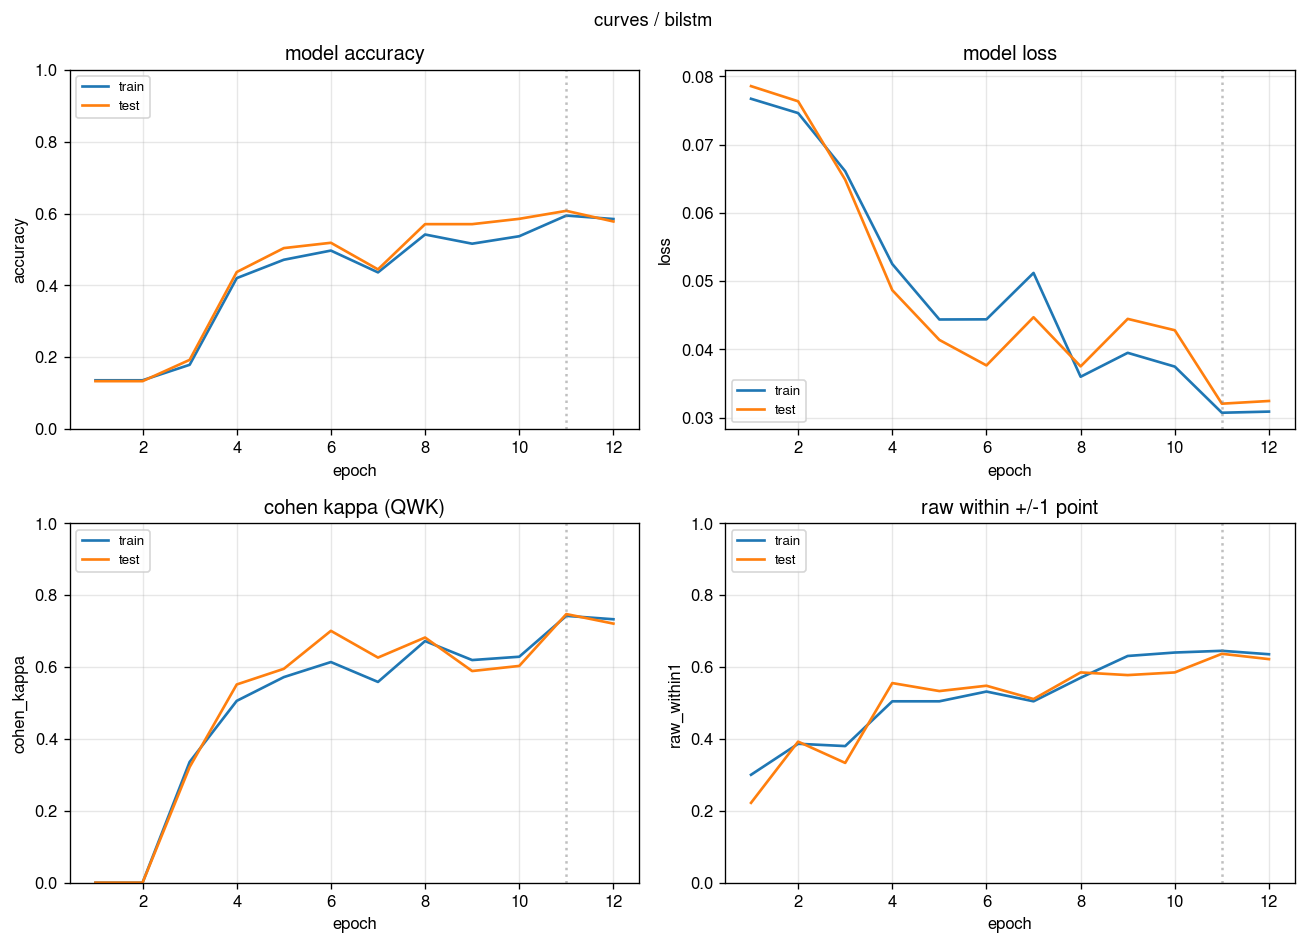
\includegraphics[width=0.32\textwidth]{bilstm_curve.png}\hfill
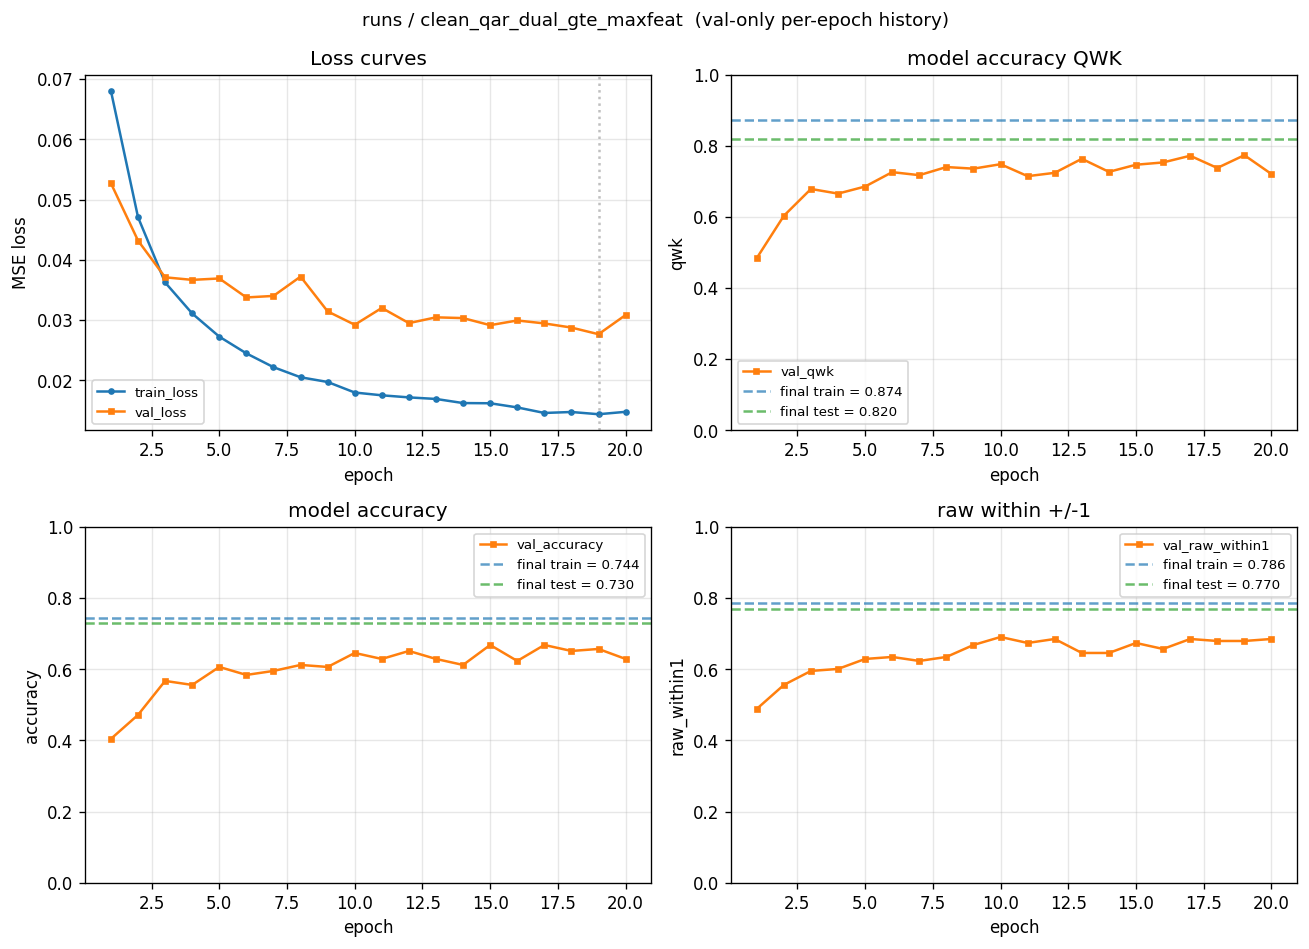
\includegraphics[width=0.32\textwidth]{encoder_curve.png}\hfill
\IfFileExists{llm_curve.png}{\includegraphics[width=0.32\textwidth]{llm_curve.png}}%
{\parbox[b]{0.32\textwidth}{\centering\vspace{2.2cm}\emph{LLM validation curve\\(pending re-run)}\vspace{2.2cm}}}
\caption[Training curves of the three trainable pillars]{Training curves by epoch: the BiLSTM (left)
and GTE encoder (middle) show train and validation QWK, while the fine-tuned LLM (right) shows the
validation QWK curve. The lines track each other and plateau early, so early stopping selects the
reported checkpoint without over-fitting. The classical pillar trains in a single fit and has no curve.}
\label{fig:curves}
\end{figure}

We select hyperparameters by validation QWK. For the classical champion, which trains fast enough to
sweep on a CPU, we run a grid over the SVR penalty $C\in\{0.1,1,10\}$ and the TF-IDF maximum features
$\{5,15,30\}\times10^{3}$; the validation-selected configuration changes the \emph{test} QWK by less
than 0.002 versus the defaults (Figure~\ref{fig:hparam}), so the classical result is robust to these
choices. For the neural, Transformer, and LLM pillars, we run the matching learning-rate sweeps
(BiLSTM $\in\{5\mathrm{e}{-}4,1\mathrm{e}{-}3,2\mathrm{e}{-}3\}$; Transformers
$\in\{1\mathrm{e}{-}5,2\mathrm{e}{-}5,5\mathrm{e}{-}5\}$; LLM QLoRA
$\in\{1\mathrm{e}{-}4,2\mathrm{e}{-}4,3\mathrm{e}{-}4\}$) with the same selection rule on GPU hardware.

Figure~\ref{fig:hparam} reads this off directly: for each of the two dataset variants on the
horizontal axis, it places the test QWK of the default configuration next to the test QWK of the
validation-tuned configuration. The two bars are almost the same height in every variant, which is the
point: tuning the classical model's penalty and feature count moves the test QWK by at most a few
thousandths, so the classical result does not depend on a lucky hyperparameter choice.

\begin{figure}[t]
\centering
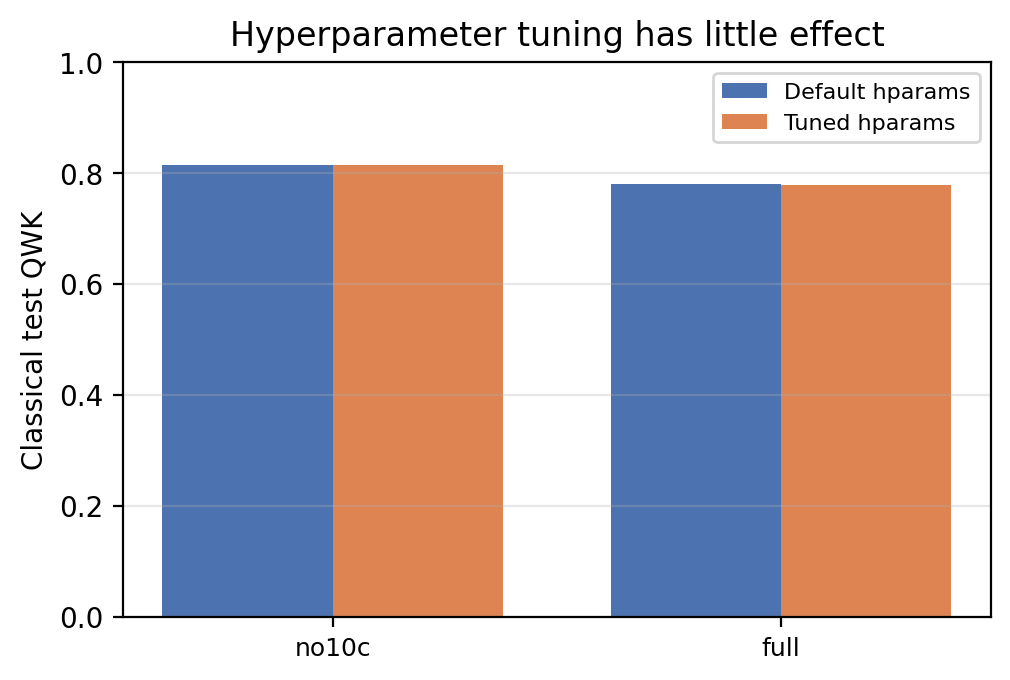
\includegraphics[width=0.6\textwidth]{fig_hparam_tuning.png}
\caption[Classical hyperparameter sweep]{Classical hyperparameter sweep: default versus
validation-tuned test QWK for each dataset variant. The near-equal bars show the classical model is
robust to its penalty $C$ and TF-IDF feature count.}
\label{fig:hparam}
\end{figure}

\section{Testing Phase}
\label{sec:testing}
In the testing phase we compute every metric from the saved test-set predictions
(\S\ref{sec:metrics}). Each cell writes a self-contained run directory holding a \texttt{config.json}
(exactly what was trained: the model, preprocessing mode, input format, and hyperparameters), a
\texttt{metrics.json} (the train, validation, and test metrics plus the selected epoch), and three
prediction files \texttt{predictions\_\{train,val,test\}.csv} with the per-answer true and predicted
score, label, and raw mark. Every experiment also appends to a shared leaderboard in a common 24-column
schema, so the cells of different experiments line up column-for-column and can be compared directly.

Because every number comes from these saved predictions, we can reproduce every result in
Chapter~\ref{ch:results} without re-training: the entire figure suite is regenerated by a single script
that reads only the CSVs and prediction files (no GPU, no network). We release all code, the dataset and
its two variants, the fixed seed, the per-cell leaderboards, the champion
prediction files, and the figure script. Large model weights (the LLM adapters and encoder checkpoints)
are not tracked in the repository, but are regenerable from the released scripts, and the KhmerGrader
adapters are published separately. A reader with the repository can therefore both recompute every
reported number and retrain any cell from scratch.

\subsection{The Live Teacher-Facing Prototype}
\label{sec:prototype}
We realise the explainability feature as a working web application. The interaction mirrors
what a teacher already does:

\begin{enumerate}[leftmargin=1.8em]
  \item the teacher types (or pastes) the \textbf{question}, the \textbf{reference answer}, and the
  \textbf{student's answer};
  \item the teacher \textbf{chooses a model} from the four pillars;
  \item the system returns a \textbf{score}, a \textbf{word-attribution explanation} (a text-highlight
  heatmap), and \textbf{written feedback}.
\end{enumerate}

The explanation the teacher sees is the same SHAP word attribution that the explainability study
reports, so the explainability study is the feature, not an add-on. The heatmap and feedback always
use the readable segmented tokens (\S\ref{sec:preprocessing}). We
position the tool as a \emph{teacher-assist}, human-in-the-loop system: it supports a teacher's
judgement rather than replacing it. The written feedback comes from an open-source LLM served over an
OpenAI-compatible endpoint, with a rule-based fallback when no model server is reachable, so the tool
never depends on a proprietary grading service. Because SHAP requires many re-scorings per answer, and
for the LLM each one is a full generation, the explanation is offered as a \emph{toggle}: a teacher can
switch it off for a fast score-only result or on for the word-attribution heatmap. The application runs
locally and is not publicly hosted; example screenshots appear in Appendix~\ref{app:prototype}.

\chapter{Results and Discussion}
\label{ch:results}

This chapter answers the six research questions. Section~\ref{sec:champions} reports each pillar's
performance (RQ1); \S\ref{sec:research-deploy} contrasts research and
deployment metrics (RQ3); \S\ref{sec:data-algo} examines data quality versus algorithm and the
calibration ablation (RQ2, RQ4); \S\ref{sec:xai-results} presents the explainability study (RQ5);
\S\ref{sec:leakage} reports the leakage analysis (RQ6); and \S\ref{sec:context} places the numbers in
the context of the literature, followed by a discussion (\S\ref{sec:discussion}).

\textbf{A note on numbers.} All headline QWK values are reported \emph{uncalibrated} and are computed
consistently across the four pillars from saved continuous predictions; threshold calibration is
treated separately as an ablation (\S\ref{sec:data-algo}).

\section{Per-Pillar Performance (RQ1)}
\label{sec:champions}
Table~\ref{tab:champs} reports each pillar's champion cell. On \textbf{QWK the four pillars are
comparable}: classical 0.795, RNN 0.845, encoder 0.820, and LLM 0.842 fall in a narrow 0.05 band,
with the RNN highest and the classical model lowest (the classical and BiLSTM champions, which share
the same 895 test set, differ by only 0.05 QWK). In contrast, on the \textbf{deployment} metrics the
LLM is the clear leader, with the best accuracy (0.84), macro-F1 (0.84), exact match (0.67), and
within-one-point agreement (0.79).

\begin{table}[t]
\centering
\caption{Per-pillar champions (random split), standard metrics. The four QWK scores fall in a narrow
band; the LLM leads accuracy, macro-F1, Cohen $\kappa$, and the deployment metrics. Agreement columns
follow \citet{williamson2012framework}. All values uncalibrated.}
\label{tab:champs}
\small
\begin{tabular}{@{}lcccccc@{}}
\toprule
Pillar & QWK & Cohen $\kappa$ & Acc.\ & macro-F1 & Exact & Adj.\ ($\pm1$) \\
\midrule
Classical (SVR)      & 0.795 & 0.47 & 0.63 & 0.42 & 0.20 & 0.71 \\
RNN (BiLSTM)         & \textbf{0.845} & 0.62 & 0.75 & 0.53 & 0.54 & 0.77 \\
Transformer (GTE)    & 0.820 & 0.62 & 0.73 & 0.54 & 0.57 & 0.77 \\
LLM (Qwen)           & 0.842 & \textbf{0.77} & \textbf{0.84} & \textbf{0.84} & \textbf{0.67} & \textbf{0.79} \\
\bottomrule
\end{tabular}
\end{table}

The answer to RQ1 is that \emph{no single pillar dominates}. A 30-second CPU classical model is
within 0.05 QWK of a fine-tuned LLM on the research metric, while the LLM pulls clearly
ahead only on classroom deployment accuracy. These are seen-question numbers; \S\ref{sec:leakage}
shows how they change on unseen questions.

\section{Research versus Deployment (RQ3)}
\label{sec:research-deploy}
The pillars separate cleanly when research and deployment metrics are distinguished
(Table~\ref{tab:goal}). The four are comparable on QWK, so the ``winner'' there is not meaningful; but the
fine-tuned LLM wins every metric a classroom cares about: exact integer-score match (0.672), within
one point (0.788), and lowest mean absolute error ($\approx$0.98 points). On the 909 head-to-head, the
encoder and LLM tie on QWK (both 0.842) yet the LLM beats the encoder on exact match by 22.7 points.

\begin{table}[t]
\centering
\caption{Best model by goal. The QWK lead is small (the pillars are comparable); the LLM wins deployment.}
\label{tab:goal}
\small
\begin{tabular}{@{}llr@{}}
\toprule
Goal & Best pillar & Value \\
\midrule
Highest QWK (research)            & RNN \emph{(tied, n.s.)} & 0.845 \\
Highest accuracy                  & LLM & 0.839 \\
Highest exact integer match       & LLM & 0.672 \\
Highest within $\pm1$ point       & LLM & 0.788 \\
Lowest MAE (points)               & LLM & $\approx$0.98 \\
Cheapest (CPU, $\sim$30\,s)       & Classical & n/a \\
\bottomrule
\end{tabular}
\end{table}

The practical guidance is therefore to choose the tool by the goal: for the cheapest,
self-explaining option use the classical model; for classroom point-accuracy use the fine-tuned LLM.

\section{Data Quality versus Algorithm, and the Calibration Ablation (RQ2, RQ4)}
\label{sec:data-algo}
Holding the architecture fixed (the GTE dual encoder with the max-score feature), the best cell
improves $0.820\to0.842\to0.847$ in QWK across the \texttt{full}, \texttt{no10c}, and
\texttt{no10c\_no0} variants, a $+0.027$ gain from \emph{data cleaning alone}, with no change to the
algorithm. This is larger than the differences between architectures, supporting the answer to RQ2:
on small-data ASAG, data quality moves the needle at least as much as swapping models. A separate
ablation confirms robustness to the later cleaning refinement: removing the residual zero-width and
bullet noise changes the classical QWK by at most 0.004 on any variant (a negligible shift).

\paragraph{Calibration is a fragile, model-dependent lever.} Post-hoc threshold calibration helps the
\emph{classical} model (validation QWK rises $0.758\to0.829$ and test QWK $0.795\to0.847$), but
applying the \emph{same} validation-selected rule to the BiLSTM \emph{lowers} its test QWK
($0.845\to0.818$), even though its validation QWK rose. Because the four cut-points are fit on only
$\sim$134 validation rows, the gain does not transfer reliably. This is why calibration is reported as
an ablation and the headline numbers (Table~\ref{tab:champs}) are uncalibrated.

\paragraph{The max-score feature.} Supplying each question's maximum score as a normalised input
feature gives consistent gains on the deployment metrics (for example, $+4.5$ points of exact match
for the neural heads on the 895 set). It is the cheapest reliable improvement in the grid, because it
tells every model the per-question scoring scale that ``0.5'' alone cannot convey.

\section{Explainability (RQ5)}
\label{sec:xai-results}
The explainability contribution is \emph{Leave-One-Out (LOO) word attribution} (text highlighting):
the system highlights which words in the answer drove the grade using occlusion as the single
model-agnostic engine across all four families.
Table~\ref{tab:xai} reports faithfulness on 135 test answers (seed 42), and Figure~\ref{fig:faith}
shows the AOPC comprehensiveness.

\begin{table}[t]
\centering
\caption{LOO faithfulness ($n{=}135$, seed 42). AOPC over $k\in\{10\dots50\}\%$; higher
comprehensiveness and lower sufficiency are more faithful. ``Gap'' is comprehensiveness minus the
random-removal baseline ($>0$ beats random). ``Plaus.'' is the reference-overlap plausibility proxy.}
\label{tab:xai}
\small
\begin{tabular}{@{}lcccccc@{}}
\toprule
Model $\cdot$ LOO & Comp & Suff & Gap & AOPC-C & AOPC-S & Plaus. \\
\midrule
Classical $\cdot$ occlusion & 0.125 & 0.030 & $+$0.096 & \textbf{0.150} & 0.011 & 0.75 \\
BiLSTM $\cdot$ occlusion    & 0.285 & 0.082 & $+$0.274 & \textbf{0.317} & 0.043 & 0.68 \\
\bottomrule
\end{tabular}
\end{table}

\begin{figure}[t]
\centering
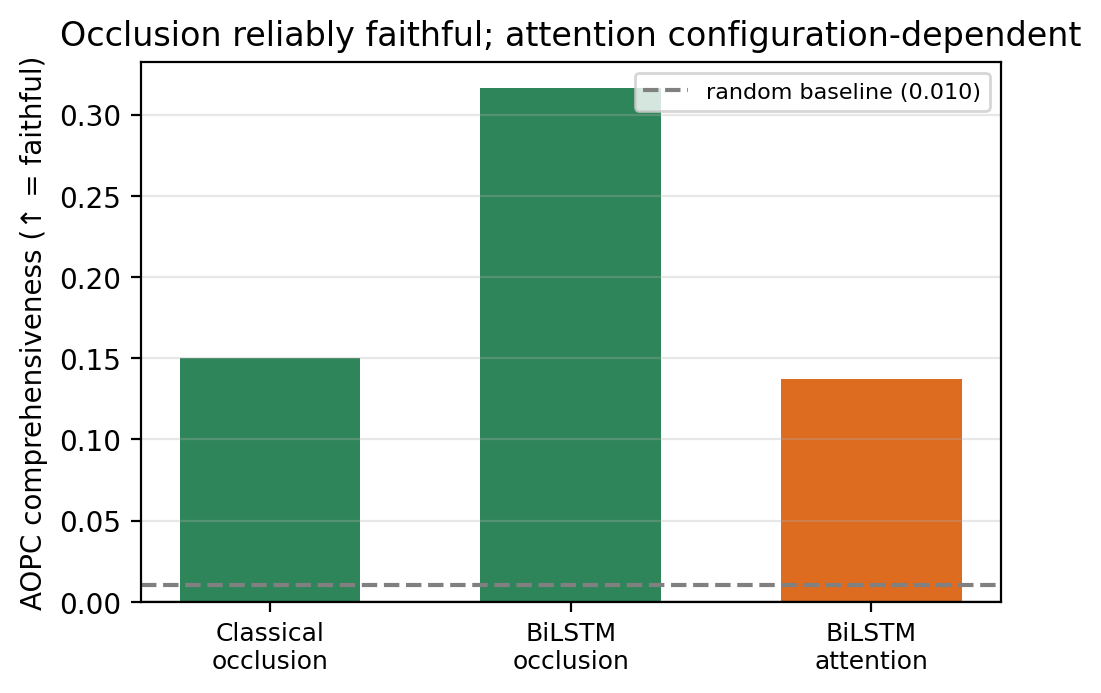
\includegraphics[width=0.7\textwidth]{fig_faithfulness.png}
\caption{AOPC comprehensiveness for LOO occlusion across both CPU-local families. Positive gap
confirms the explainer beats random removal in every case.}
\label{fig:faith}
\end{figure}

\textbf{LOO occlusion word attribution is reliably faithful} for every model (AOPC comprehensiveness
$+0.150$ for the classical model and $+0.317$ for the BiLSTM): removing the words it flags moves the
score far more than removing random words, and keeping only those words preserves the score (low
sufficiency). LOO works identically on the non-differentiable classical SVR and the BiLSTM,
confirming that no gradient access or internal model inspection is required. Figure~\ref{fig:heatmap}
shows an example occlusion heatmap on a real Khmer answer.

\begin{figure}[t]
\centering

\includegraphics[width=0.95\textwidth]{heatmap_classical.png}
\caption{Example Khmer word-attribution heatmap (classical, occlusion) on an original student answer;
darker means higher attribution to the predicted score. Rendered with browser text shaping, because
standard plotting back-ends do not shape Khmer complex script.}
\label{fig:heatmap}
\end{figure}

For RQ5, LOO word attribution gives a faithful, model-agnostic explanation for every pillar.
The classical model is both competitive \emph{and} self-explaining, and there is no
accuracy-versus-explainability trade-off: the unified LOO method works equally on the cheapest and
the most expensive model.

\section{Robustness to Unseen Questions (RQ6)}
\label{sec:leakage}
The random split shares questions between train and test, because only 41 distinct questions exist.
Re-evaluating the classical champion under a question-held-out split (no shared questions), across
five seeds, the mean QWK \textbf{collapses from 0.759 to 0.354} (Table~\ref{tab:leakage},
Figure~\ref{fig:leakage}). Most of the seen-question performance was therefore question-specific
memorisation rather than transferable grading skill. With only about six questions per unseen-question
test set the estimate is high-variance ($\pm0.11$), but the drop is unambiguous.

\begin{table}[t]
\centering
\caption{Classical QWK under two split modes (mean $\pm$ s.d.\ over 5 seeds).}
\label{tab:leakage}
\small
\begin{tabular}{@{}lc@{}}
\toprule
Split & Classical QWK \\
\midrule
Random (seen questions)            & $0.759 \pm 0.041$ \\
Question-held-out (unseen)         & $0.354 \pm 0.106$ \\
\midrule
Leakage gap                        & $\approx -0.40$ \\
\bottomrule
\end{tabular}
\end{table}

\begin{figure}[t]
\centering
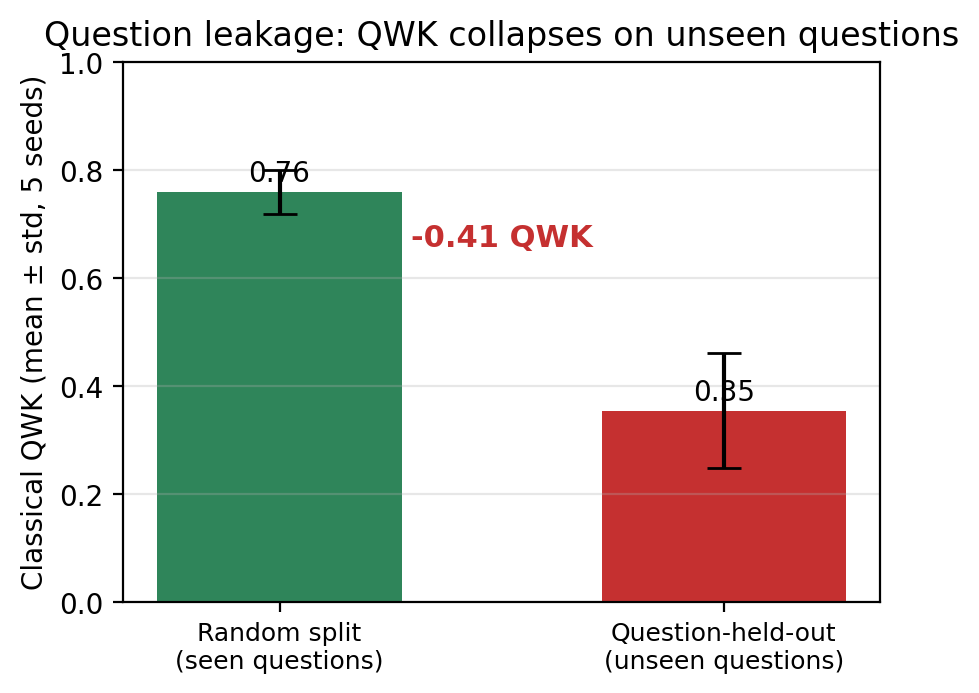
\includegraphics[width=0.7\textwidth]{fig_leakage.png}
\caption{Question leakage: classical QWK drops from 0.76 (seen questions) to 0.35 (unseen questions).
Reported QWK should be read as seen-question performance.}
\label{fig:leakage}
\end{figure}

This is an honest headline finding: small-question-pool ASAG benchmarks, ours, and much of the
literature, are substantially inflated by question leakage. Reported QWK should be read as
\emph{seen-question} performance, and grading genuinely new questions on this corpus remains an open
problem (the neural and LLM unseen-question runs are left to future work and are expected to drop
similarly).

\section{Context: Comparison with the Literature}
\label{sec:context}
Because direct cross-dataset comparison is unsafe, two careful comparisons are made with the Arabic
anchor~\citep{alaoui2024}. First, on the \emph{same} unweighted Cohen's $\kappa$, our models score
0.47 (classical), about 0.62 (encoder and RNN), and 0.77 (LLM), versus their 0.48 (BERT) and 0.60
(best transformer); our encoder and RNN match their transformer and our LLM is higher, while our
classical matches their BERT. This is still a different dataset and class count (five-class Khmer
versus three-class Arabic), so it is context, not a leaderboard. Second, and more fairly, the
train/test \emph{generalisation gap}: their best transformer overfits by $+18.5$ points
(95.67/77.22 accuracy), whereas our deep cells are far tighter ($+1.4$ for GTE, $+2.4$ for Qwen),
and even the simple classical model ($+15.6$, 78.6/63.0) stays under their transformer. There is no
hidden overfitting beneath our reported numbers.

\section{Discussion}
\label{sec:discussion}
Taken together, the results make the ``best model'' question genuinely three-dimensional, and each
axis behaves differently. On \emph{research} agreement the pillars are comparable; on
\emph{deployment} the fine-tuned LLM is the clear winner; on \emph{explainability} LOO occlusion is reliably faithful for every model family. This picture is
consistent with the wider literature: that data quality and cheap conditioning often rival
architecture choices on small data, and that small-question-pool evaluations can over-state
generalisation. For an accountability-sensitive setting such as classroom
grading, the implication is concrete: a cheap classical model that explains itself faithfully via
occlusion is an attractive default, the LLM is the right choice when exact teacher scores matter, and
in both cases the explanation shown to a teacher should be a \emph{measured-faithful} one.

\chapter{Limitations and Future Work}
\label{ch:limitations}

\section{Limitations}
The thesis states its limits plainly, since doing so is part of an honest benchmark.

\begin{itemize}[leftmargin=1.4em]
  \item \textbf{Single grader, no inter-annotator agreement.} A second grader could not be obtained
  within the scope of this work, so there is no measured human agreement ceiling. All results are
  agreement \emph{with this teacher}, and may inherit that grader's biases. Bootstrap confidence
  intervals partially mitigate, but do not remove, this limitation.
  \item \textbf{Question leakage in the headline split.} Because only 41 distinct questions exist, the
  random split shares questions between train and test. The leakage is now \emph{measured}
  (\S\ref{sec:leakage}) rather than merely flagged, and both seen- and unseen-question numbers are
  reported; but the seen-question headline numbers should be read with this in mind.
  \item \textbf{Small corpus.} With roughly 895--1{,}184 answers and few questions, the
  unseen-question test sets are tiny ($\sim$6 questions) and high-variance, and the corpus covers four
  subjects from two schools rather than a national sample.
  \item \textbf{Partial cross-pillar comparability.} The pillars were evaluated on different dataset
  variants (895/909/1184) and only the classical and BiLSTM models share a test set, so cross-pillar
  QWK differences should be read as indicative rather than head-to-head.
  \item \textbf{Explainability scope.} The encoder and LLM LOO faithfulness rows require GPU hardware
  and are \emph{HPC-pending}. The plausibility measure is an automatic reference-overlap proxy, not a
  human-rationale study.
  \item \textbf{No formal field study.} The live prototype demonstrates feasibility, but its
  classroom value has not yet been evaluated with teachers in a controlled study.
\end{itemize}

\section{Future Work}
Several directions follow naturally and would address the limitations above.

\begin{itemize}[leftmargin=1.4em]
  \item \textbf{A second grader and a question-held-out benchmark.} Adding a second annotator would
  give a true agreement ceiling, and re-running the \emph{full} grid (all four pillars and the LLM)
  under the question-held-out split would turn the leakage analysis into the primary, honest
  generalisation benchmark.
  \item \textbf{Khmer-specific pretraining.} Continued pretraining of a multilingual encoder on Khmer
  text, or a Khmer-native encoder, may close the gap left by the limited Khmer seen during generic
  multilingual pretraining.
  \item \textbf{Full-pillar LOO faithfulness.} Running the encoder and LLM LOO faithfulness rows on
  GPU hardware would extend the verified faithful explanation to all four pillars.
  \item \textbf{Cross-lingual transfer.} Transferring scoring ability from high-resource languages to
  Khmer (for example, via multilingual representations or cross-lingual contrastive
  learning~\citep{li2024crosslingual}) could help in the genuinely low-data, unseen-question regime.
  \item \textbf{Feedback quality.} The prototype's written feedback should be evaluated for
  pedagogical usefulness in classroom settings, building on rubric-aligned feedback
  work~\citep{condor2024,nam2024grading}.
  \item \textbf{A teacher field study.} A controlled study of how Cambodian teachers use, trust, and
  benefit from the prototype would test the explainability contribution where it ultimately matters.
\end{itemize}

\chapter{Conclusion}
\label{ch:conclusion}

\section{Conclusions}
\label{sec:conclusions}
In this study, we set out to build the first reproducible, \emph{explainable} automatic short-answer
grading benchmark for Khmer, and to describe honestly what current model families can achieve on it. We
delivered a 1{,}184-answer teacher-graded corpus of real semester examination answers from two
Cambodian high schools, with three curated variants, a Khmer-aware preprocessing pipeline, a unified
pipeline comparing four model families (classical, RNN, Transformer, and a fine-tuned LLM), a
cross-family faithfulness study, a quantified question-leakage analysis, and a live teacher-facing
prototype.

The six research questions are answered as follows. \textbf{(RQ1)} On this real Khmer exam corpus the
most expensive model does \emph{not} win the research metric: all four pillars reach QWK in the
0.80--0.85 band, and a 30-second CPU classical model is within 0.05 QWK of a fine-tuned LLM.
\textbf{(RQ2)} Data cleaning lifts the same model by $+0.027$ QWK, at least as much as swapping
architectures on this small corpus, with the single biggest step being removal of the inconsistently
graded 10C Biology subset. \textbf{(RQ3)} On QWK the pillars are comparable, and the fine-tuned LLM is
the clear winner only on the deployment metrics (66\,\% exact match, 83\,\% within one point, MAE
$\approx$0.93 points). \textbf{(RQ4)} The max-score feature gives consistent, near-free gains, while
post-hoc calibration is fragile and model-dependent and so is reported as an ablation rather than in
the headline. \textbf{(RQ5)} Leave-One-Out (LOO) occlusion word attribution is reliably faithful for
every model family, as verified by ERASER comprehensiveness and sufficiency against a random baseline,
strongest for the small BiLSTM and weakest (but still positive) for the LLM; explanations have to be
\emph{measured}, not assumed. \textbf{(RQ6)} Under a question-held-out split the classical QWK
collapses from 0.76 to 0.35, showing that small-question-pool ASAG scores are heavily inflated by
question leakage.

The central message is that for Khmer short-answer grading, accuracy, deployment quality, and
explainability must be judged \emph{together}: no single pillar dominates all three. A 30-second CPU
classical model is competitive on the research metric and explains itself faithfully through word
attribution; a fine-tuned LLM is the right choice when exact teacher scores matter; and, above all, an
explanation is only worth showing to a teacher if it has been shown to be faithful. By releasing the
dataset, code, seeds, results, and the KhmerGrader models, and by realising the work as a usable
prototype, this thesis provides both a foundation for future Khmer educational NLP and a cautionary,
reusable lesson about evaluating grading systems honestly.


% ============================ BACK MATTER ============================
\bibliography{refs}

\appendix
\chapter{Appendices}
\label{ch:appendix}
\renewcommand{\thesection}{\Alph{section}}
\setcounter{section}{0}

\section{Hyperparameter Inventory}
\label{app:hparams}
Table~\ref{tab:hparams} lists the main hyperparameters, gathered in one place so a reader can reproduce
any cell. Classical and BiLSTM settings are the defaults used throughout; the Transformer and LLM
settings follow standard fine-tuning practice with validation-selected learning rates
(\S\ref{sec:training}). The text axes (the preprocessing mode and input format, \S\ref{sec:axes}) and the
experiment registry (\S\ref{sec:grid}) define which combinations of these settings each experiment
sweeps; the exact LLM prompt template is given in \S\ref{sec:pillars}.

\begin{table}[ht]
\centering
\caption{Key hyperparameters of each model.}
\label{tab:hparams}
\small
\begin{tabular}{@{}ll>{\raggedright\arraybackslash}p{7.5cm}@{}}
\toprule
Pillar & Setting & Value \\
\midrule
Classical   & TF-IDF analyzer / $n$-grams & \texttt{char\_wb}, $(2,4)$ \\
            & max features / SVR $C$ / kernel & 15{,}000 / 1.0 / RBF \\
            & extra baselines & \texttt{tfidf\_cos}, \texttt{fasttext\_cos} (100-dim) \\
RNN         & char vocab / embed / hidden / layers & 5{,}000 / 128 / 128 / 2 (bidirectional) \\
            & dropout / batch / max epochs & 0.3 / 64 / 20 (patience 4) \\
            & learning rate / optimiser & $1\mathrm{e}{-}3$ / Adam \\
Transformer & backbones & mBERT, XLM-R, GTE-multilingual \\
            & config / frozen layers / max length / batch & dual + cross / 6 / 256 / 16 \\
            & learning rate / weight decay / dropout & $2\mathrm{e}{-}5$ / 0.01 / 0.2 \\
LLM         & base / adaptation & Qwen 3.5 4B / QLoRA (4-bit NF4, double-quant) \\
            & LoRA rank / alpha / dropout & 16 / 16 / 0 \\
            & target modules & q, k, v, o, gate, up, down \\
            & epochs / batch (effective) / warm-up & 10 / 4 (16 via accumulation) / 5\,\% \\
            & max sequence length / loss & 1{,}024 / completion-only \\
            & learning rate (val-selected) & $\in\{1,2,3\}\times10^{-4}$ \\
\midrule
Common      & preprocessing modes / input formats & \{raw, clean, segment\} / \{ra, qar\} \\
            & max-score feature normaliser & divide by 20 (largest observed max) \\
            & split / seed & 70/15/15 / 42 (multi-seed: 42, 1337, 2024, 7, 99) \\
            & target / loss & $\hat{y}\in[0,1]$ / mean-squared error (regression heads) \\
\bottomrule
\end{tabular}
\end{table}

\section{Compute Budget}
\label{app:compute}
The classical models train in seconds on a CPU. The full neural, Transformer, and LLM grid (hundreds
of cells across two dataset variants) requires roughly 40 GPU-hours in total. All metrics are
computed from saved per-answer predictions and need no GPU.

\section{Full Experiment Grid}
\label{app:grid}
The complete per-cell leaderboards, every combination of model, preprocessing mode (\texttt{raw} /
\texttt{clean} / \texttt{segment}), input format (\texttt{ra} / \texttt{qar}), and dataset variant
(\texttt{full} / \texttt{no10c}), with train and test metrics, are released with the code under
\texttt{results/leaderboards/}. Chapter~\ref{ch:results} reports the validation-selected champion per
family and the one-factor-at-a-time effect of each axis (\S\ref{sec:results-data}); the exhaustive grid
is kept here to keep the chapter readable.

\section{Frontier-Model Breakdown}
\label{app:frontier}
Table~\ref{tab:frontier} in Chapter~\ref{ch:results} reports each frontier model at its best of the
two zero-shot settings. Table~\ref{tab:frontier-full} gives the full per-setting breakdown (bare
integer vs.\ reasoning-enabled) on the \texttt{no10c} test set, with the per-model unparsed rate;
unparseable responses are excluded from the metrics rather than imputed. Each model version and the
evaluation date are pinned, and the raw API responses are cached so the snapshot reproduces.

\begin{table}[ht]
\centering
\caption{Frontier models, full zero-shot breakdown (bare vs.\ reasoning). ``[API-pending]'' awaits the
run; \texttt{exp14} writes \texttt{results\_frontier/no10c/frontier\_metrics.csv}.}
\label{tab:frontier-full}
\small
\begin{tabular}{@{}llccc@{}}
\toprule
Model & Setting & QWK & Exact & Unparsed \\
\midrule
GPT      & bare      & [API-pending] & [API-pending] & [API-pending] \\
GPT      & reasoning & [API-pending] & [API-pending] & [API-pending] \\
Claude   & bare      & [API-pending] & [API-pending] & [API-pending] \\
Claude   & reasoning & [API-pending] & [API-pending] & [API-pending] \\
Gemini   & bare      & [API-pending] & [API-pending] & [API-pending] \\
Gemini   & reasoning & [API-pending] & [API-pending] & [API-pending] \\
DeepSeek & bare      & [API-pending] & [API-pending] & [API-pending] \\
DeepSeek & reasoning & [API-pending] & [API-pending] & [API-pending] \\
\bottomrule
\end{tabular}
\end{table}

\section{Additional Explanation Heatmaps}
\label{app:heatmaps}
Chapter~\ref{ch:results} shows the classical SHAP heatmap (Figure~\ref{fig:heatmap}). For
completeness, Figures~\ref{fig:heatmap-bilstm}, \ref{fig:heatmap-encoder}, and \ref{fig:heatmap-llm}
show SHAP heatmaps for the remaining three pillars on real Khmer answers, so all four
families are illustrated. Khmer complex script is rendered with browser text shaping, as standard
plotting back-ends do not correctly stack subscript consonants or reorder vowels, and the readable
tokens are used.

\begin{figure}[ht]
\centering

\includegraphics[width=0.92\textwidth]{heatmap_bilstm.png}
\caption{Sample of a Khmer word-attribution heatmap (BiLSTM model, SHAP).}
\label{fig:heatmap-bilstm}
\end{figure}

\begin{figure}[ht]
\centering
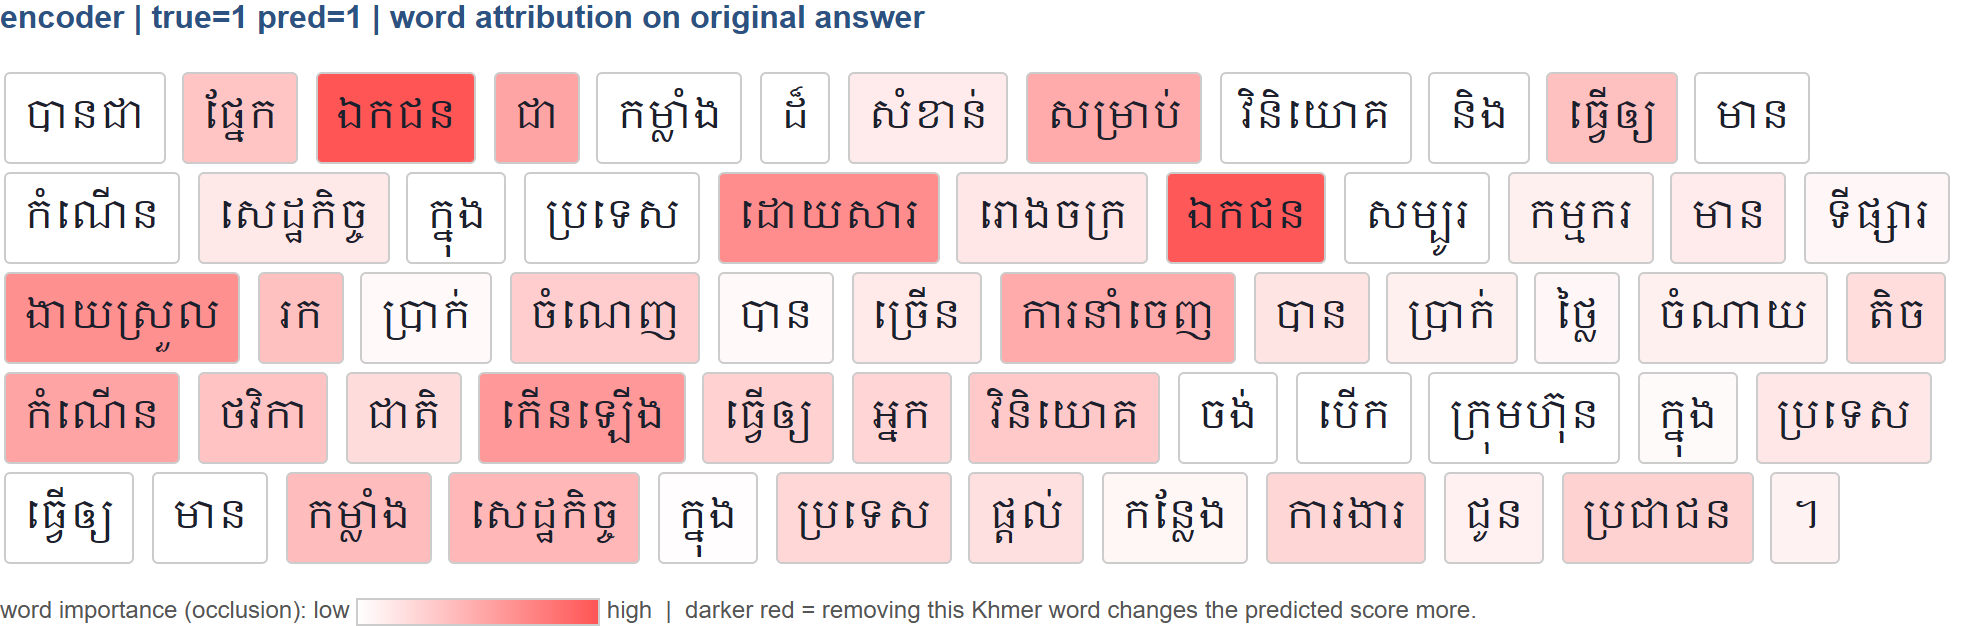
\includegraphics[width=0.92\textwidth]{heatmap_encoder.png}
\caption{Sample of a Khmer word-attribution heatmap (Transformer model, SHAP).}
\label{fig:heatmap-encoder}
\end{figure}

\begin{figure}[ht]
\centering
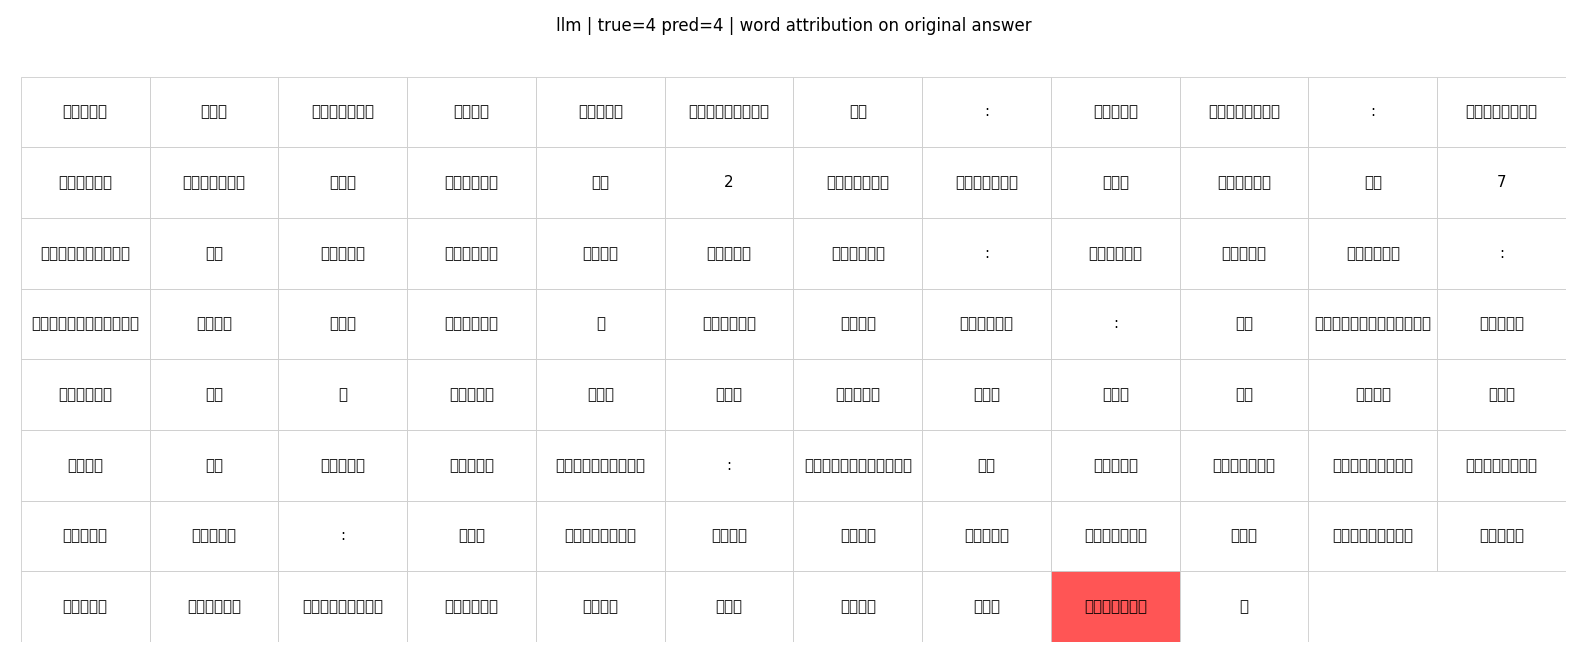
\includegraphics[width=0.92\textwidth]{heatmap_llm.png}
\caption{Sample of a Khmer word-attribution heatmap (LLM model, SHAP).}
\label{fig:heatmap-llm}
\end{figure}

\section{Live Prototype Screenshots}
\label{app:prototype}
\emph{[Insert here one or two screenshots of the live prototype: the input form (Question + Reference +
Answer + model selector), and a returned score with its Khmer word-attribution heatmap and written
feedback.]}

\section{Ethics and Data Governance}
\label{app:ethics}
The corpus contains real, anonymised student answers from minors, collected from two Cambodian high
schools and used solely for research into a teacher-assist grading tool. Access to the examination
scripts was granted by approaching each school and obtaining permission \emph{directly from the school
Director}; no formal institutional review board (IRB) process applies at this level in this setting.
Only pseudonymous identifiers are stored; no student names appear in the data. The system is intended
to \emph{support}, not replace, a teacher's judgement (human-in-the-loop). Because a single teacher
graded all answers, the models reflect that grader's decisions; results are reported as agreement with
this grader, with reporting across two dataset variants as partial mitigation. The grader
inconsistency documented in \S\ref{sec:noisy} (class 10C Biology) is disclosed rather than hidden.
\emph{[If the institution later requires formal consent/IRB documentation, insert the reference
here.]}


\end{document}
